\documentclass[twoside]{book}

% Packages required by doxygen
\usepackage{calc}
\usepackage{doxygen}
\usepackage{graphicx}
\usepackage[utf8]{inputenc}
\usepackage{makeidx}
\usepackage{multicol}
\usepackage{multirow}
\usepackage{textcomp}
\usepackage[table]{xcolor}

% Font selection
\usepackage[T1]{fontenc}
\usepackage{mathptmx}
\usepackage[scaled=.90]{helvet}
\usepackage{courier}
\usepackage{amssymb}
\usepackage{sectsty}
\renewcommand{\familydefault}{\sfdefault}
\allsectionsfont{%
  \fontseries{bc}\selectfont%
  \color{darkgray}%
}
\renewcommand{\DoxyLabelFont}{%
  \fontseries{bc}\selectfont%
  \color{darkgray}%
}

% Page & text layout
\usepackage{geometry}
\geometry{%
  a4paper,%
  top=2.5cm,%
  bottom=2.5cm,%
  left=2.5cm,%
  right=2.5cm%
}
\tolerance=750
\hfuzz=15pt
\hbadness=750
\setlength{\emergencystretch}{15pt}
\setlength{\parindent}{0cm}
\setlength{\parskip}{0.2cm}
\makeatletter
\renewcommand{\paragraph}{%
  \@startsection{paragraph}{4}{0ex}{-1.0ex}{1.0ex}{%
    \normalfont\normalsize\bfseries\SS@parafont%
  }%
}
\renewcommand{\subparagraph}{%
  \@startsection{subparagraph}{5}{0ex}{-1.0ex}{1.0ex}{%
    \normalfont\normalsize\bfseries\SS@subparafont%
  }%
}
\makeatother

% Headers & footers
\usepackage{fancyhdr}
\pagestyle{fancyplain}
\fancyhead[LE]{\fancyplain{}{\bfseries\thepage}}
\fancyhead[CE]{\fancyplain{}{}}
\fancyhead[RE]{\fancyplain{}{\bfseries\leftmark}}
\fancyhead[LO]{\fancyplain{}{\bfseries\rightmark}}
\fancyhead[CO]{\fancyplain{}{}}
\fancyhead[RO]{\fancyplain{}{\bfseries\thepage}}
\fancyfoot[LE]{\fancyplain{}{}}
\fancyfoot[CE]{\fancyplain{}{}}
\fancyfoot[RE]{\fancyplain{}{\bfseries\scriptsize Generated on Sat Oct 26 2013 12\-:38\-:31 for F\-F\-X\-I\-V\-L\-I\-B by Doxygen }}
\fancyfoot[LO]{\fancyplain{}{\bfseries\scriptsize Generated on Sat Oct 26 2013 12\-:38\-:31 for F\-F\-X\-I\-V\-L\-I\-B by Doxygen }}
\fancyfoot[CO]{\fancyplain{}{}}
\fancyfoot[RO]{\fancyplain{}{}}
\renewcommand{\footrulewidth}{0.4pt}
\renewcommand{\chaptermark}[1]{%
  \markboth{#1}{}%
}
\renewcommand{\sectionmark}[1]{%
  \markright{\thesection\ #1}%
}

% Indices & bibliography
\usepackage{natbib}
\usepackage[titles]{tocloft}
\setcounter{tocdepth}{3}
\setcounter{secnumdepth}{5}
\makeindex

% Hyperlinks (required, but should be loaded last)
\usepackage{ifpdf}
\ifpdf
  \usepackage[pdftex,pagebackref=true]{hyperref}
\else
  \usepackage[ps2pdf,pagebackref=true]{hyperref}
\fi
\hypersetup{%
  colorlinks=true,%
  linkcolor=blue,%
  citecolor=blue,%
  unicode%
}

% Custom commands
\newcommand{\clearemptydoublepage}{%
  \newpage{\pagestyle{empty}\cleardoublepage}%
}


%===== C O N T E N T S =====

\begin{document}

% Titlepage & ToC
\hypersetup{pageanchor=false}
\pagenumbering{roman}
\begin{titlepage}
\vspace*{7cm}
\begin{center}%
{\Large F\-F\-X\-I\-V\-L\-I\-B }\\
\vspace*{1cm}
{\large Generated by Doxygen 1.8.5}\\
\vspace*{0.5cm}
{\small Sat Oct 26 2013 12:38:31}\\
\end{center}
\end{titlepage}
\clearemptydoublepage
\tableofcontents
\clearemptydoublepage
\pagenumbering{arabic}
\hypersetup{pageanchor=true}

%--- Begin generated contents ---
\chapter{ffxivlib}
\label{md__r_e_a_d_m_e}
\hypertarget{md__r_e_a_d_m_e}{}
\input{md__r_e_a_d_m_e}
\chapter{Namespace Index}
\section{Packages}
Here are the packages with brief descriptions (if available)\-:\begin{DoxyCompactList}
\item\contentsline{section}{\hyperlink{namespaceffxivlib}{ffxivlib} }{\pageref{namespaceffxivlib}}{}
\end{DoxyCompactList}

\chapter{Hierarchical Index}
\section{Class Hierarchy}
This inheritance list is sorted roughly, but not completely, alphabetically\-:\begin{DoxyCompactList}
\item \contentsline{section}{ffxivlib.\-Chatlog.\-C\-H\-A\-T\-L\-O\-G\-I\-N\-F\-O}{\pageref{structffxivlib_1_1_chatlog_1_1_c_h_a_t_l_o_g_i_n_f_o}}{}
\item \contentsline{section}{ffxivlib.\-Movement\-Helper.\-Coords}{\pageref{structffxivlib_1_1_movement_helper_1_1_coords}}{}
\item \contentsline{section}{ffxivlib.\-Entity.\-E\-N\-T\-I\-T\-Y\-I\-N\-F\-O}{\pageref{structffxivlib_1_1_entity_1_1_e_n_t_i_t_y_i_n_f_o}}{}
\item \contentsline{section}{ffxivlib.\-Chatlog.\-Entry}{\pageref{classffxivlib_1_1_chatlog_1_1_entry}}{}
\item \contentsline{section}{ffxivlib.\-F\-F\-X\-I\-V\-L\-I\-B}{\pageref{classffxivlib_1_1_f_f_x_i_v_l_i_b}}{}
\item \contentsline{section}{ffxivlib.\-I\-Container$<$ T, U $>$}{\pageref{classffxivlib_1_1_i_container_3_01_t_00_01_u_01_4}}{}
\begin{DoxyCompactList}
\item \contentsline{section}{ffxivlib.\-Chatlog}{\pageref{classffxivlib_1_1_chatlog}}{}
\item \contentsline{section}{ffxivlib.\-Entity}{\pageref{classffxivlib_1_1_entity}}{}
\item \contentsline{section}{ffxivlib.\-Party\-Member}{\pageref{classffxivlib_1_1_party_member}}{}
\item \contentsline{section}{ffxivlib.\-Player}{\pageref{classffxivlib_1_1_player}}{}
\item \contentsline{section}{ffxivlib.\-Target}{\pageref{classffxivlib_1_1_target}}{}
\end{DoxyCompactList}
\item \contentsline{section}{ffxivlib.\-Movement\-Helper}{\pageref{classffxivlib_1_1_movement_helper}}{}
\item \contentsline{section}{ffxivlib.\-Party\-Member.\-P\-A\-R\-T\-Y\-M\-E\-M\-B\-E\-R\-I\-N\-F\-O}{\pageref{structffxivlib_1_1_party_member_1_1_p_a_r_t_y_m_e_m_b_e_r_i_n_f_o}}{}
\item \contentsline{section}{ffxivlib.\-Player.\-P\-L\-A\-Y\-E\-R\-I\-N\-F\-O}{\pageref{structffxivlib_1_1_player_1_1_p_l_a_y_e_r_i_n_f_o}}{}
\item \contentsline{section}{ffxivlib.\-Send\-Key\-Input}{\pageref{classffxivlib_1_1_send_key_input}}{}
\item \contentsline{section}{ffxivlib.\-Party\-Member.\-S\-T\-A\-T\-U\-S\-E\-F\-F\-E\-C\-T}{\pageref{structffxivlib_1_1_party_member_1_1_s_t_a_t_u_s_e_f_f_e_c_t}}{}
\item \contentsline{section}{ffxivlib.\-Target.\-T\-A\-R\-G\-E\-T}{\pageref{structffxivlib_1_1_target_1_1_t_a_r_g_e_t}}{}
\end{DoxyCompactList}

\chapter{Class Index}
\section{Class List}
Here are the classes, structs, unions and interfaces with brief descriptions\-:\begin{DoxyCompactList}
\item\contentsline{section}{\hyperlink{structffxivlib_1_1_b_u_f_f}{ffxivlib.\-B\-U\-F\-F} }{\pageref{structffxivlib_1_1_b_u_f_f}}{}
\item\contentsline{section}{\hyperlink{class_resources_dumper_1_1_buff}{Resources\-Dumper.\-Buff} }{\pageref{class_resources_dumper_1_1_buff}}{}
\item\contentsline{section}{\hyperlink{classffxivlib_1_1_chatlog}{ffxivlib.\-Chatlog} }{\pageref{classffxivlib_1_1_chatlog}}{}
\item\contentsline{section}{\hyperlink{structffxivlib_1_1_chatlog_1_1_c_h_a_t_l_o_g_i_n_f_o}{ffxivlib.\-Chatlog.\-C\-H\-A\-T\-L\-O\-G\-I\-N\-F\-O} }{\pageref{structffxivlib_1_1_chatlog_1_1_c_h_a_t_l_o_g_i_n_f_o}}{}
\item\contentsline{section}{\hyperlink{structffxivlib_1_1_movement_helper_1_1_coords}{ffxivlib.\-Movement\-Helper.\-Coords} }{\pageref{structffxivlib_1_1_movement_helper_1_1_coords}}{}
\item\contentsline{section}{\hyperlink{classffxivlib_1_1_entity}{ffxivlib.\-Entity} }{\pageref{classffxivlib_1_1_entity}}{}
\item\contentsline{section}{\hyperlink{structffxivlib_1_1_entity_1_1_e_n_t_i_t_y_i_n_f_o}{ffxivlib.\-Entity.\-E\-N\-T\-I\-T\-Y\-I\-N\-F\-O} }{\pageref{structffxivlib_1_1_entity_1_1_e_n_t_i_t_y_i_n_f_o}}{}
\item\contentsline{section}{\hyperlink{classffxivlib_1_1_chatlog_1_1_entry}{ffxivlib.\-Chatlog.\-Entry} }{\pageref{classffxivlib_1_1_chatlog_1_1_entry}}{}
\item\contentsline{section}{\hyperlink{classffxivlib_1_1_f_f_x_i_v_l_i_b}{ffxivlib.\-F\-F\-X\-I\-V\-L\-I\-B} }{\pageref{classffxivlib_1_1_f_f_x_i_v_l_i_b}}{}
\item\contentsline{section}{\hyperlink{classffxivlib_1_1_i_container_3_01_t_00_01_u_01_4}{ffxivlib.\-I\-Container$<$ T, U $>$} \\*Basic managed container for structures and other infos }{\pageref{classffxivlib_1_1_i_container_3_01_t_00_01_u_01_4}}{}
\item\contentsline{section}{\hyperlink{classffxivlib_1_1_inventory}{ffxivlib.\-Inventory} }{\pageref{classffxivlib_1_1_inventory}}{}
\item\contentsline{section}{\hyperlink{structffxivlib_1_1_inventory_1_1_i_n_v_e_n_t_o_r_y}{ffxivlib.\-Inventory.\-I\-N\-V\-E\-N\-T\-O\-R\-Y} \\*Structure holding all the pointers to different subarrays. }{\pageref{structffxivlib_1_1_inventory_1_1_i_n_v_e_n_t_o_r_y}}{}
\item\contentsline{section}{\hyperlink{classffxivlib_1_1_inventory_1_1_inventory_builder}{ffxivlib.\-Inventory.\-Inventory\-Builder} \\*Basic container for our list of items. }{\pageref{classffxivlib_1_1_inventory_1_1_inventory_builder}}{}
\item\contentsline{section}{\hyperlink{structffxivlib_1_1_inventory_1_1_i_t_e_m}{ffxivlib.\-Inventory.\-I\-T\-E\-M} \\*Structure representing an item }{\pageref{structffxivlib_1_1_inventory_1_1_i_t_e_m}}{}
\item\contentsline{section}{\hyperlink{classffxivlib_1_1_movement_helper}{ffxivlib.\-Movement\-Helper} \\*Credits to F\-F\-A\-C\-E\-T\-O\-O\-L\-S. }{\pageref{classffxivlib_1_1_movement_helper}}{}
\item\contentsline{section}{\hyperlink{classffxivlib_1_1_party_member}{ffxivlib.\-Party\-Member} }{\pageref{classffxivlib_1_1_party_member}}{}
\item\contentsline{section}{\hyperlink{structffxivlib_1_1_party_member_1_1_p_a_r_t_y_m_e_m_b_e_r_i_n_f_o}{ffxivlib.\-Party\-Member.\-P\-A\-R\-T\-Y\-M\-E\-M\-B\-E\-R\-I\-N\-F\-O} }{\pageref{structffxivlib_1_1_party_member_1_1_p_a_r_t_y_m_e_m_b_e_r_i_n_f_o}}{}
\item\contentsline{section}{\hyperlink{classffxivlib_1_1_player}{ffxivlib.\-Player} }{\pageref{classffxivlib_1_1_player}}{}
\item\contentsline{section}{\hyperlink{structffxivlib_1_1_player_1_1_p_l_a_y_e_r_i_n_f_o}{ffxivlib.\-Player.\-P\-L\-A\-Y\-E\-R\-I\-N\-F\-O} }{\pageref{structffxivlib_1_1_player_1_1_p_l_a_y_e_r_i_n_f_o}}{}
\item\contentsline{section}{\hyperlink{class_get_inventory_1_1_program}{Get\-Inventory.\-Program} }{\pageref{class_get_inventory_1_1_program}}{}
\item\contentsline{section}{\hyperlink{class_dump_inventory_1_1_program}{Dump\-Inventory.\-Program} }{\pageref{class_dump_inventory_1_1_program}}{}
\item\contentsline{section}{\hyperlink{class_resources_dumper_1_1_program}{Resources\-Dumper.\-Program} }{\pageref{class_resources_dumper_1_1_program}}{}
\item\contentsline{section}{\hyperlink{class_get_gathering_nodes_1_1_program}{Get\-Gathering\-Nodes.\-Program} }{\pageref{class_get_gathering_nodes_1_1_program}}{}
\item\contentsline{section}{\hyperlink{class_constants_1_1_resource_parser}{Constants.\-Resource\-Parser} \\*Some parameters can be overriden B\-E\-F\-O\-R\-E instanciating F\-F\-X\-I\-V\-L\-I\-B. }{\pageref{class_constants_1_1_resource_parser}}{}
\item\contentsline{section}{\hyperlink{classffxivlib_1_1_send_key_input}{ffxivlib.\-Send\-Key\-Input} }{\pageref{classffxivlib_1_1_send_key_input}}{}
\item\contentsline{section}{\hyperlink{class_serializable_dictionary_3_01_t_key_00_01_t_value_01_4}{Serializable\-Dictionary$<$ T\-Key, T\-Value $>$} }{\pageref{class_serializable_dictionary_3_01_t_key_00_01_t_value_01_4}}{}
\item\contentsline{section}{\hyperlink{class_s_q_lite_database}{S\-Q\-Lite\-Database} }{\pageref{class_s_q_lite_database}}{}
\item\contentsline{section}{\hyperlink{structffxivlib_1_1_target_1_1_t_a_r_g_e_t}{ffxivlib.\-Target.\-T\-A\-R\-G\-E\-T} }{\pageref{structffxivlib_1_1_target_1_1_t_a_r_g_e_t}}{}
\item\contentsline{section}{\hyperlink{classffxivlib_1_1_target}{ffxivlib.\-Target} }{\pageref{classffxivlib_1_1_target}}{}
\end{DoxyCompactList}

\chapter{Namespace Documentation}
\hypertarget{namespace_current_target}{\section{Package Current\-Target}
\label{namespace_current_target}\index{Current\-Target@{Current\-Target}}
}
\subsection*{Classes}
\begin{DoxyCompactItemize}
\item 
class \hyperlink{class_current_target_1_1_program}{Program}
\end{DoxyCompactItemize}

\hypertarget{namespaceffxivlib}{\section{Package ffxivlib}
\label{namespaceffxivlib}\index{ffxivlib@{ffxivlib}}
}
\subsection*{Classes}
\begin{DoxyCompactItemize}
\item 
class \hyperlink{classffxivlib_1_1_base_object_3_01_t_u_01_4}{Base\-Object$<$ T\-U $>$}
\begin{DoxyCompactList}\small\item\em Abstract base class for various objects \end{DoxyCompactList}\item 
struct \hyperlink{structffxivlib_1_1_b_u_f_f}{B\-U\-F\-F}
\item 
class \hyperlink{classffxivlib_1_1_chatlog}{Chatlog}
\item 
class \hyperlink{classffxivlib_1_1_f_f_x_i_v_l_i_b}{F\-F\-X\-I\-V\-L\-I\-B}
\item 
class \hyperlink{classffxivlib_1_1_companion}{Companion}
\item 
class \hyperlink{classffxivlib_1_1_entity}{Entity}
\item 
class \hyperlink{classffxivlib_1_1_inventory}{Inventory}
\item 
class {\bfseries Library}
\item 
class {\bfseries Memory\-Reader}
\item 
class \hyperlink{classffxivlib_1_1_movement_helper}{Movement\-Helper}
\begin{DoxyCompactList}\small\item\em Credits to F\-F\-A\-C\-E\-T\-O\-O\-L\-S. \end{DoxyCompactList}\item 
class \hyperlink{classffxivlib_1_1_party_member}{Party\-Member}
\item 
class \hyperlink{classffxivlib_1_1_player}{Player}
\item 
class {\bfseries Resource\-Parser}
\item 
class \hyperlink{classffxivlib_1_1_send_key_input}{Send\-Key\-Input}
\item 
class {\bfseries Serializer}
\item 
class {\bfseries Sig\-Scanner}
\item 
class \hyperlink{classffxivlib_1_1_target}{Target}
\end{DoxyCompactItemize}
\subsection*{Enumerations}
\begin{DoxyCompactItemize}
\item 
enum \hyperlink{namespaceffxivlib_a7273810711af045adb7151580e025a86}{J\-O\-B} \-: byte \{ \\*
{\bfseries G\-L\-D} = 0x1, 
{\bfseries P\-G\-L} = 0x2, 
{\bfseries M\-R\-D} = 0x3, 
{\bfseries L\-N\-C} = 0x4, 
\\*
{\bfseries A\-R\-C} = 0x5, 
{\bfseries C\-N\-J} = 0x6, 
{\bfseries T\-H\-M} = 0x7, 
{\bfseries C\-P\-T} = 0x8, 
\\*
{\bfseries B\-S\-M} = 0x9, 
{\bfseries A\-R\-M} = 0x\-A, 
{\bfseries G\-S\-M} = 0x\-B, 
{\bfseries L\-T\-W} = 0x\-C, 
\\*
{\bfseries W\-V\-R} = 0x\-D, 
{\bfseries A\-L\-C} = 0x\-E, 
{\bfseries C\-U\-L} = 0x\-F, 
{\bfseries M\-I\-N} = 0x10, 
\\*
{\bfseries B\-O\-T} = 0x11, 
{\bfseries F\-S\-H} = 0x12, 
{\bfseries P\-L\-D} = 0x13, 
{\bfseries M\-N\-K} = 0x14, 
\\*
{\bfseries W\-A\-R} = 0x15, 
{\bfseries D\-R\-G} = 0x16, 
{\bfseries B\-R\-D} = 0x17, 
{\bfseries W\-H\-M} = 0x18, 
\\*
{\bfseries B\-L\-M} = 0x19, 
{\bfseries A\-C\-N} = 0x2\-A, 
{\bfseries S\-M\-N} = 0x2\-B, 
{\bfseries S\-C\-H} = 0x2\-C, 
\\*
{\bfseries Chocobo} = 0x2\-D, 
{\bfseries Pet} = 0x2\-E
 \}
\begin{DoxyCompactList}\small\item\em Job I\-D as used in various structures \end{DoxyCompactList}\item 
enum {\bfseries S\-E\-X} \-: byte \{ {\bfseries Male} = 0x0, 
{\bfseries Female} = 0x1
 \}
\item 
enum \hyperlink{namespaceffxivlib_a93f054414b7ccf7ba7c36f54fcc392f5}{E\-N\-T\-I\-T\-Y\-S\-T\-A\-T\-U\-S} \-: byte \{ \\*
{\bfseries Idle} = 0x01, 
{\bfseries Dead} = 0x02, 
{\bfseries Sitting} = 0x03, 
{\bfseries Mounted} = 0x04, 
\\*
{\bfseries Crafting} = 0x05, 
{\bfseries Gathering} = 0x06, 
{\bfseries Melding} = 0x07, 
{\bfseries S\-Machine} = 0x08
 \}
\begin{DoxyCompactList}\small\item\em Current action of an Entity (P\-C) \end{DoxyCompactList}\item 
enum \hyperlink{namespaceffxivlib_a856915176aeab1f9b643c0243cb008ee}{S\-T\-A\-T\-U\-S} \-: byte \{ {\bfseries Engaged} = 0x01, 
{\bfseries Idle} = 0x02, 
{\bfseries Crafting} = 0x05
 \}
\begin{DoxyCompactList}\small\item\em Status of an Entity (P\-C/\-N\-P\-C) \end{DoxyCompactList}\item 
enum \hyperlink{namespaceffxivlib_aaa4e86d1ea6dbc1661147e6616256e68}{T\-Y\-P\-E} \-: byte \{ \\*
{\bfseries Player} = 0x01, 
{\bfseries Mob} = 0x02, 
{\bfseries N\-P\-C} = 0x03, 
{\bfseries Aetheryte} = 0x05, 
\\*
{\bfseries Gathering} = 0x06, 
{\bfseries Minion} = 0x09
 \}
\begin{DoxyCompactList}\small\item\em Type of the entity \end{DoxyCompactList}\item 
enum \hyperlink{namespaceffxivlib_a3a6b3a65a3fc9ba42586b2ccc07e4aac}{I\-C\-O\-N} \-: byte \{ \\*
{\bfseries None} = 0x0, 
{\bfseries Yoshida} = 0x1, 
{\bfseries G\-M} = 0x2, 
{\bfseries S\-G\-M} = 0x3, 
\\*
{\bfseries Clover} = 0x4, 
{\bfseries Dc} = 0x5, 
{\bfseries Smiley} = 0x6, 
{\bfseries Red\-Cross} = 0x9, 
\\*
{\bfseries Grey\-Dc} = 0x\-A, 
{\bfseries Processing} = 0x\-B, 
{\bfseries Busy} = 0x\-C, 
{\bfseries Duty} = 0x\-D, 
\\*
{\bfseries Processing\-Yellow} = 0x\-E, 
{\bfseries Processing\-Grey} = 0x\-F, 
{\bfseries Cutscene} = 0x10, 
{\bfseries Chocobo} = 0x12, 
\\*
{\bfseries Sitting} = 0x13, 
{\bfseries Wrench\-Yellow} = 0x14, 
{\bfseries Wrench} = 0x15, 
{\bfseries Dice} = 0x16, 
\\*
{\bfseries Processing\-Green} = 0x17, 
{\bfseries Sword} = 0x18, 
{\bfseries Duty\-Finder} = 0x19, 
{\bfseries Alliance\-Leader} = 0x1\-A, 
\\*
{\bfseries Alliance\-Blue\-Leader} = 0x1\-B, 
{\bfseries Alliance\-Blue} = 0x1\-C, 
{\bfseries Sprout} = 0x1\-F, 
{\bfseries Gil} = 0x20
 \}
\begin{DoxyCompactList}\small\item\em Icons \end{DoxyCompactList}\item 
enum \hyperlink{namespaceffxivlib_a027fd426531e3a42243f5c2b946dde31}{C\-U\-R\-R\-E\-N\-T\-T\-A\-R\-G\-E\-T} \-: byte \{ {\bfseries Own} = 0x1, 
{\bfseries True} = 0x2, 
{\bfseries False} = 0x4
 \}
\begin{DoxyCompactList}\small\item\em Because S\-E likes to use values that don't make sense. \end{DoxyCompactList}\item 
enum \hyperlink{namespaceffxivlib_a08bcc753fec0a3174d818ecaa25aec4f}{E\-Q\-U\-I\-P\-\_\-\-P\-O\-S} \-: byte \{ \\*
{\bfseries Main\-Hand} = 0, 
{\bfseries Off\-Hand} = 1, 
{\bfseries Head} = 2, 
{\bfseries Body} = 3, 
\\*
{\bfseries Hands} = 4, 
{\bfseries Waist} = 5, 
{\bfseries Legs} = 6, 
{\bfseries Feet} = 7, 
\\*
{\bfseries Neck} = 8, 
{\bfseries Ears} = 9, 
{\bfseries Wrists} = 10, 
{\bfseries Left\-Ring} = 11, 
\\*
{\bfseries Right\-Ring} = 12, 
{\bfseries Soul\-Crystal} = 13
 \}
\begin{DoxyCompactList}\small\item\em This is used for get\-Current\-Equipment() \end{DoxyCompactList}\end{DoxyCompactItemize}


\subsection{Enumeration Type Documentation}
\hypertarget{namespaceffxivlib_a027fd426531e3a42243f5c2b946dde31}{\index{ffxivlib@{ffxivlib}!C\-U\-R\-R\-E\-N\-T\-T\-A\-R\-G\-E\-T@{C\-U\-R\-R\-E\-N\-T\-T\-A\-R\-G\-E\-T}}
\index{C\-U\-R\-R\-E\-N\-T\-T\-A\-R\-G\-E\-T@{C\-U\-R\-R\-E\-N\-T\-T\-A\-R\-G\-E\-T}!ffxivlib@{ffxivlib}}
\subsubsection[{C\-U\-R\-R\-E\-N\-T\-T\-A\-R\-G\-E\-T}]{\setlength{\rightskip}{0pt plus 5cm}enum {\bf ffxivlib.\-C\-U\-R\-R\-E\-N\-T\-T\-A\-R\-G\-E\-T} \-: byte}}\label{namespaceffxivlib_a027fd426531e3a42243f5c2b946dde31}


Because S\-E likes to use values that don't make sense. 

\hypertarget{namespaceffxivlib_a93f054414b7ccf7ba7c36f54fcc392f5}{\index{ffxivlib@{ffxivlib}!E\-N\-T\-I\-T\-Y\-S\-T\-A\-T\-U\-S@{E\-N\-T\-I\-T\-Y\-S\-T\-A\-T\-U\-S}}
\index{E\-N\-T\-I\-T\-Y\-S\-T\-A\-T\-U\-S@{E\-N\-T\-I\-T\-Y\-S\-T\-A\-T\-U\-S}!ffxivlib@{ffxivlib}}
\subsubsection[{E\-N\-T\-I\-T\-Y\-S\-T\-A\-T\-U\-S}]{\setlength{\rightskip}{0pt plus 5cm}enum {\bf ffxivlib.\-E\-N\-T\-I\-T\-Y\-S\-T\-A\-T\-U\-S} \-: byte}}\label{namespaceffxivlib_a93f054414b7ccf7ba7c36f54fcc392f5}


Current action of an \hyperlink{classffxivlib_1_1_entity}{Entity} (P\-C) 

\hypertarget{namespaceffxivlib_a08bcc753fec0a3174d818ecaa25aec4f}{\index{ffxivlib@{ffxivlib}!E\-Q\-U\-I\-P\-\_\-\-P\-O\-S@{E\-Q\-U\-I\-P\-\_\-\-P\-O\-S}}
\index{E\-Q\-U\-I\-P\-\_\-\-P\-O\-S@{E\-Q\-U\-I\-P\-\_\-\-P\-O\-S}!ffxivlib@{ffxivlib}}
\subsubsection[{E\-Q\-U\-I\-P\-\_\-\-P\-O\-S}]{\setlength{\rightskip}{0pt plus 5cm}enum {\bf ffxivlib.\-E\-Q\-U\-I\-P\-\_\-\-P\-O\-S} \-: byte}}\label{namespaceffxivlib_a08bcc753fec0a3174d818ecaa25aec4f}


This is used for get\-Current\-Equipment() 

\hypertarget{namespaceffxivlib_a3a6b3a65a3fc9ba42586b2ccc07e4aac}{\index{ffxivlib@{ffxivlib}!I\-C\-O\-N@{I\-C\-O\-N}}
\index{I\-C\-O\-N@{I\-C\-O\-N}!ffxivlib@{ffxivlib}}
\subsubsection[{I\-C\-O\-N}]{\setlength{\rightskip}{0pt plus 5cm}enum {\bf ffxivlib.\-I\-C\-O\-N} \-: byte}}\label{namespaceffxivlib_a3a6b3a65a3fc9ba42586b2ccc07e4aac}


Icons 

\hypertarget{namespaceffxivlib_a7273810711af045adb7151580e025a86}{\index{ffxivlib@{ffxivlib}!J\-O\-B@{J\-O\-B}}
\index{J\-O\-B@{J\-O\-B}!ffxivlib@{ffxivlib}}
\subsubsection[{J\-O\-B}]{\setlength{\rightskip}{0pt plus 5cm}enum {\bf ffxivlib.\-J\-O\-B} \-: byte}}\label{namespaceffxivlib_a7273810711af045adb7151580e025a86}


Job I\-D as used in various structures 

\hypertarget{namespaceffxivlib_a856915176aeab1f9b643c0243cb008ee}{\index{ffxivlib@{ffxivlib}!S\-T\-A\-T\-U\-S@{S\-T\-A\-T\-U\-S}}
\index{S\-T\-A\-T\-U\-S@{S\-T\-A\-T\-U\-S}!ffxivlib@{ffxivlib}}
\subsubsection[{S\-T\-A\-T\-U\-S}]{\setlength{\rightskip}{0pt plus 5cm}enum {\bf ffxivlib.\-S\-T\-A\-T\-U\-S} \-: byte}}\label{namespaceffxivlib_a856915176aeab1f9b643c0243cb008ee}


Status of an \hyperlink{classffxivlib_1_1_entity}{Entity} (P\-C/\-N\-P\-C) 

\hypertarget{namespaceffxivlib_aaa4e86d1ea6dbc1661147e6616256e68}{\index{ffxivlib@{ffxivlib}!T\-Y\-P\-E@{T\-Y\-P\-E}}
\index{T\-Y\-P\-E@{T\-Y\-P\-E}!ffxivlib@{ffxivlib}}
\subsubsection[{T\-Y\-P\-E}]{\setlength{\rightskip}{0pt plus 5cm}enum {\bf ffxivlib.\-T\-Y\-P\-E} \-: byte}}\label{namespaceffxivlib_aaa4e86d1ea6dbc1661147e6616256e68}


Type of the entity 


\hypertarget{namespace_modify_icon}{\section{Package Modify\-Icon}
\label{namespace_modify_icon}\index{Modify\-Icon@{Modify\-Icon}}
}
\subsection*{Classes}
\begin{DoxyCompactItemize}
\item 
class \hyperlink{class_modify_icon_1_1_program}{Program}
\end{DoxyCompactItemize}

\chapter{Class Documentation}
\hypertarget{classffxivlib_1_1_entity}{\section{ffxivlib.\-Entity Class Reference}
\label{classffxivlib_1_1_entity}\index{ffxivlib.\-Entity@{ffxivlib.\-Entity}}
}
Inheritance diagram for ffxivlib.\-Entity\-:\begin{figure}[H]
\begin{center}
\leavevmode
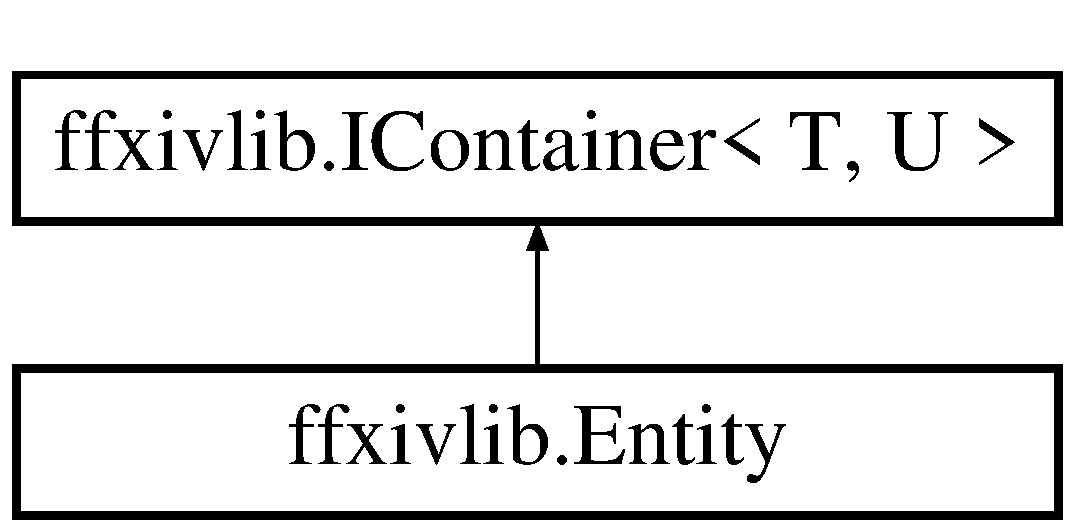
\includegraphics[height=2.000000cm]{classffxivlib_1_1_entity}
\end{center}
\end{figure}
\subsection*{Classes}
\begin{DoxyCompactItemize}
\item 
struct \hyperlink{structffxivlib_1_1_entity_1_1_e_n_t_i_t_y_i_n_f_o}{E\-N\-T\-I\-T\-Y\-I\-N\-F\-O}
\end{DoxyCompactItemize}
\subsection*{Public Member Functions}
\begin{DoxyCompactItemize}
\item 
\hypertarget{classffxivlib_1_1_entity_ad8f9917fb98bf79a98427972aae4a0f5}{{\bfseries Entity} (\hyperlink{structffxivlib_1_1_entity_1_1_e_n_t_i_t_y_i_n_f_o}{E\-N\-T\-I\-T\-Y\-I\-N\-F\-O} \-\_\-structure, Int\-Ptr \-\_\-address)}\label{classffxivlib_1_1_entity_ad8f9917fb98bf79a98427972aae4a0f5}

\end{DoxyCompactItemize}
\subsection*{Additional Inherited Members}


The documentation for this class was generated from the following file\-:\begin{DoxyCompactItemize}
\item 
Entity.\-cs\end{DoxyCompactItemize}

\hypertarget{structffxivlib_1_1_entity_1_1_e_n_t_i_t_y_i_n_f_o}{\section{ffxivlib.\-Entity.\-E\-N\-T\-I\-T\-Y\-I\-N\-F\-O Struct Reference}
\label{structffxivlib_1_1_entity_1_1_e_n_t_i_t_y_i_n_f_o}\index{ffxivlib.\-Entity.\-E\-N\-T\-I\-T\-Y\-I\-N\-F\-O@{ffxivlib.\-Entity.\-E\-N\-T\-I\-T\-Y\-I\-N\-F\-O}}
}
\subsection*{Public Attributes}
\begin{DoxyCompactItemize}
\item 
\hypertarget{structffxivlib_1_1_entity_1_1_e_n_t_i_t_y_i_n_f_o_a179e48b58b038509c996fd001b630450}{int {\bfseries Gathering\-Type}}\label{structffxivlib_1_1_entity_1_1_e_n_t_i_t_y_i_n_f_o_a179e48b58b038509c996fd001b630450}

\item 
\hypertarget{structffxivlib_1_1_entity_1_1_e_n_t_i_t_y_i_n_f_o_a6e5d16391e1a4c5315d62bedb8adc6ee}{string {\bfseries Name}}\label{structffxivlib_1_1_entity_1_1_e_n_t_i_t_y_i_n_f_o_a6e5d16391e1a4c5315d62bedb8adc6ee}

\item 
\hypertarget{structffxivlib_1_1_entity_1_1_e_n_t_i_t_y_i_n_f_o_afa12b9fce3ef427e77dbc4959323da85}{int {\bfseries P\-C\-Id}}\label{structffxivlib_1_1_entity_1_1_e_n_t_i_t_y_i_n_f_o_afa12b9fce3ef427e77dbc4959323da85}

\item 
\hypertarget{structffxivlib_1_1_entity_1_1_e_n_t_i_t_y_i_n_f_o_ab314a76301cf72f6db84632975204195}{int {\bfseries N\-P\-C\-Id}}\label{structffxivlib_1_1_entity_1_1_e_n_t_i_t_y_i_n_f_o_ab314a76301cf72f6db84632975204195}

\item 
\hypertarget{structffxivlib_1_1_entity_1_1_e_n_t_i_t_y_i_n_f_o_a42fd66513e50082589fa96b06b8bb5ca}{\hyperlink{namespaceffxivlib_aaa4e86d1ea6dbc1661147e6616256e68}{T\-Y\-P\-E} {\bfseries Mob\-Type}}\label{structffxivlib_1_1_entity_1_1_e_n_t_i_t_y_i_n_f_o_a42fd66513e50082589fa96b06b8bb5ca}

\item 
\hypertarget{structffxivlib_1_1_entity_1_1_e_n_t_i_t_y_i_n_f_o_aabe85fc004243fb307da9691578df5b3}{\hyperlink{namespaceffxivlib_a027fd426531e3a42243f5c2b946dde31}{C\-U\-R\-R\-E\-N\-T\-T\-A\-R\-G\-E\-T} {\bfseries Current\-Target}}\label{structffxivlib_1_1_entity_1_1_e_n_t_i_t_y_i_n_f_o_aabe85fc004243fb307da9691578df5b3}

\item 
\hypertarget{structffxivlib_1_1_entity_1_1_e_n_t_i_t_y_i_n_f_o_a553a0320ee3e9ef52e5771fee99b2f2e}{byte {\bfseries Distance}}\label{structffxivlib_1_1_entity_1_1_e_n_t_i_t_y_i_n_f_o_a553a0320ee3e9ef52e5771fee99b2f2e}

\item 
\hypertarget{structffxivlib_1_1_entity_1_1_e_n_t_i_t_y_i_n_f_o_a773d937c244ff15ff7d5aa68d1083dc5}{byte {\bfseries Gathering\-Status}}\label{structffxivlib_1_1_entity_1_1_e_n_t_i_t_y_i_n_f_o_a773d937c244ff15ff7d5aa68d1083dc5}

\item 
\hypertarget{structffxivlib_1_1_entity_1_1_e_n_t_i_t_y_i_n_f_o_a6c542f7ef80b754b74031829ece457a3}{float {\bfseries X}}\label{structffxivlib_1_1_entity_1_1_e_n_t_i_t_y_i_n_f_o_a6c542f7ef80b754b74031829ece457a3}

\item 
\hypertarget{structffxivlib_1_1_entity_1_1_e_n_t_i_t_y_i_n_f_o_a557a202012e334a5fbc6173568931390}{float {\bfseries Z}}\label{structffxivlib_1_1_entity_1_1_e_n_t_i_t_y_i_n_f_o_a557a202012e334a5fbc6173568931390}

\item 
\hypertarget{structffxivlib_1_1_entity_1_1_e_n_t_i_t_y_i_n_f_o_a553962f61f6f53e475ab357a743816fb}{float {\bfseries Y}}\label{structffxivlib_1_1_entity_1_1_e_n_t_i_t_y_i_n_f_o_a553962f61f6f53e475ab357a743816fb}

\item 
\hypertarget{structffxivlib_1_1_entity_1_1_e_n_t_i_t_y_i_n_f_o_ae2653ecf98d2c097309f988cf03342c7}{float {\bfseries Heading}}\label{structffxivlib_1_1_entity_1_1_e_n_t_i_t_y_i_n_f_o_ae2653ecf98d2c097309f988cf03342c7}

\item 
\hypertarget{structffxivlib_1_1_entity_1_1_e_n_t_i_t_y_i_n_f_o_a7e7d7eb6347c20ba16f2d5057638de41}{byte {\bfseries Gathering\-Invisible}}\label{structffxivlib_1_1_entity_1_1_e_n_t_i_t_y_i_n_f_o_a7e7d7eb6347c20ba16f2d5057638de41}

\item 
\hypertarget{structffxivlib_1_1_entity_1_1_e_n_t_i_t_y_i_n_f_o_a5c70bba9773173eb899896e495d9daf4}{int {\bfseries Model\-I\-D}}\label{structffxivlib_1_1_entity_1_1_e_n_t_i_t_y_i_n_f_o_a5c70bba9773173eb899896e495d9daf4}

\item 
\hypertarget{structffxivlib_1_1_entity_1_1_e_n_t_i_t_y_i_n_f_o_a48a81848eba0a57a877e64416f8e14bd}{\hyperlink{namespaceffxivlib_a93f054414b7ccf7ba7c36f54fcc392f5}{E\-N\-T\-I\-T\-Y\-S\-T\-A\-T\-U\-S} {\bfseries Player\-Status}}\label{structffxivlib_1_1_entity_1_1_e_n_t_i_t_y_i_n_f_o_a48a81848eba0a57a877e64416f8e14bd}

\item 
\hypertarget{structffxivlib_1_1_entity_1_1_e_n_t_i_t_y_i_n_f_o_a112f53600dc197a709db1294a4ce34ef}{bool {\bfseries Is\-G\-M}}\label{structffxivlib_1_1_entity_1_1_e_n_t_i_t_y_i_n_f_o_a112f53600dc197a709db1294a4ce34ef}

\item 
\hypertarget{structffxivlib_1_1_entity_1_1_e_n_t_i_t_y_i_n_f_o_a5aaafe3d225104b151f4bcbf87806ff1}{byte {\bfseries Icon}}\label{structffxivlib_1_1_entity_1_1_e_n_t_i_t_y_i_n_f_o_a5aaafe3d225104b151f4bcbf87806ff1}

\item 
\hypertarget{structffxivlib_1_1_entity_1_1_e_n_t_i_t_y_i_n_f_o_af1e7d07d8d9ec58c1d894db8f42c8e05}{\hyperlink{namespaceffxivlib_a856915176aeab1f9b643c0243cb008ee}{S\-T\-A\-T\-U\-S} {\bfseries Is\-Engaged}}\label{structffxivlib_1_1_entity_1_1_e_n_t_i_t_y_i_n_f_o_af1e7d07d8d9ec58c1d894db8f42c8e05}

\item 
\hypertarget{structffxivlib_1_1_entity_1_1_e_n_t_i_t_y_i_n_f_o_a5037220e6d432e2fb27d089a0e33336d}{int {\bfseries Target\-Id}}\label{structffxivlib_1_1_entity_1_1_e_n_t_i_t_y_i_n_f_o_a5037220e6d432e2fb27d089a0e33336d}

\item 
\hypertarget{structffxivlib_1_1_entity_1_1_e_n_t_i_t_y_i_n_f_o_adb0f4f2a9875b4b94d7f248462f3b563}{byte {\bfseries Grand\-Company}}\label{structffxivlib_1_1_entity_1_1_e_n_t_i_t_y_i_n_f_o_adb0f4f2a9875b4b94d7f248462f3b563}

\item 
\hypertarget{structffxivlib_1_1_entity_1_1_e_n_t_i_t_y_i_n_f_o_a5d6119649d0a4e78d01cdf8fa6a1b136}{byte {\bfseries Grand\-Company\-Rank}}\label{structffxivlib_1_1_entity_1_1_e_n_t_i_t_y_i_n_f_o_a5d6119649d0a4e78d01cdf8fa6a1b136}

\item 
\hypertarget{structffxivlib_1_1_entity_1_1_e_n_t_i_t_y_i_n_f_o_adb6f8a551e474839b27f784e0b85b561}{byte {\bfseries Title}}\label{structffxivlib_1_1_entity_1_1_e_n_t_i_t_y_i_n_f_o_adb6f8a551e474839b27f784e0b85b561}

\item 
\hypertarget{structffxivlib_1_1_entity_1_1_e_n_t_i_t_y_i_n_f_o_aa61e592d9c0a60bf1853205fb977231b}{\hyperlink{namespaceffxivlib_a7273810711af045adb7151580e025a86}{J\-O\-B} {\bfseries Job}}\label{structffxivlib_1_1_entity_1_1_e_n_t_i_t_y_i_n_f_o_aa61e592d9c0a60bf1853205fb977231b}

\item 
\hypertarget{structffxivlib_1_1_entity_1_1_e_n_t_i_t_y_i_n_f_o_a4f0a0379cf62b99154f31f0429c534cf}{byte {\bfseries Level}}\label{structffxivlib_1_1_entity_1_1_e_n_t_i_t_y_i_n_f_o_a4f0a0379cf62b99154f31f0429c534cf}

\item 
\hypertarget{structffxivlib_1_1_entity_1_1_e_n_t_i_t_y_i_n_f_o_a70e57fbfa2fa3dd47e457a83180dd30b}{int {\bfseries Current\-H\-P}}\label{structffxivlib_1_1_entity_1_1_e_n_t_i_t_y_i_n_f_o_a70e57fbfa2fa3dd47e457a83180dd30b}

\item 
\hypertarget{structffxivlib_1_1_entity_1_1_e_n_t_i_t_y_i_n_f_o_a46d67cfaf28ca6236241d0980f6fac59}{int {\bfseries Max\-H\-P}}\label{structffxivlib_1_1_entity_1_1_e_n_t_i_t_y_i_n_f_o_a46d67cfaf28ca6236241d0980f6fac59}

\item 
\hypertarget{structffxivlib_1_1_entity_1_1_e_n_t_i_t_y_i_n_f_o_aa65fab657ee54589bb0744618111028d}{int {\bfseries Current\-M\-P}}\label{structffxivlib_1_1_entity_1_1_e_n_t_i_t_y_i_n_f_o_aa65fab657ee54589bb0744618111028d}

\item 
\hypertarget{structffxivlib_1_1_entity_1_1_e_n_t_i_t_y_i_n_f_o_ab55df5485ad2c251412921a74de18e94}{int {\bfseries Max\-M\-P}}\label{structffxivlib_1_1_entity_1_1_e_n_t_i_t_y_i_n_f_o_ab55df5485ad2c251412921a74de18e94}

\item 
\hypertarget{structffxivlib_1_1_entity_1_1_e_n_t_i_t_y_i_n_f_o_a0b078d43f885ea3e0e5561087a269f39}{short {\bfseries Current\-T\-P}}\label{structffxivlib_1_1_entity_1_1_e_n_t_i_t_y_i_n_f_o_a0b078d43f885ea3e0e5561087a269f39}

\item 
\hypertarget{structffxivlib_1_1_entity_1_1_e_n_t_i_t_y_i_n_f_o_a704400c457cb1ffc1b445642a4a5bd94}{short {\bfseries Current\-G\-P}}\label{structffxivlib_1_1_entity_1_1_e_n_t_i_t_y_i_n_f_o_a704400c457cb1ffc1b445642a4a5bd94}

\item 
\hypertarget{structffxivlib_1_1_entity_1_1_e_n_t_i_t_y_i_n_f_o_aac1da1a035793be9d863c15f14123355}{short {\bfseries Max\-G\-P}}\label{structffxivlib_1_1_entity_1_1_e_n_t_i_t_y_i_n_f_o_aac1da1a035793be9d863c15f14123355}

\item 
\hypertarget{structffxivlib_1_1_entity_1_1_e_n_t_i_t_y_i_n_f_o_af10df6e508ba32017c0fcd8ee1564e0a}{short {\bfseries Current\-C\-P}}\label{structffxivlib_1_1_entity_1_1_e_n_t_i_t_y_i_n_f_o_af10df6e508ba32017c0fcd8ee1564e0a}

\item 
\hypertarget{structffxivlib_1_1_entity_1_1_e_n_t_i_t_y_i_n_f_o_a27bd950cd1dfb8494cf69f89f5834e34}{short {\bfseries Max\-C\-P}}\label{structffxivlib_1_1_entity_1_1_e_n_t_i_t_y_i_n_f_o_a27bd950cd1dfb8494cf69f89f5834e34}

\item 
\hypertarget{structffxivlib_1_1_entity_1_1_e_n_t_i_t_y_i_n_f_o_a699875cd7898172929592fd6b407c68c}{byte {\bfseries Race}}\label{structffxivlib_1_1_entity_1_1_e_n_t_i_t_y_i_n_f_o_a699875cd7898172929592fd6b407c68c}

\item 
\hypertarget{structffxivlib_1_1_entity_1_1_e_n_t_i_t_y_i_n_f_o_a53d07d9b89bec006286483c633cfc616}{S\-E\-X {\bfseries Sex}}\label{structffxivlib_1_1_entity_1_1_e_n_t_i_t_y_i_n_f_o_a53d07d9b89bec006286483c633cfc616}

\item 
\hypertarget{structffxivlib_1_1_entity_1_1_e_n_t_i_t_y_i_n_f_o_afb50f40f28a62629c3efc0a1f8057615}{byte {\bfseries Aggro}}\label{structffxivlib_1_1_entity_1_1_e_n_t_i_t_y_i_n_f_o_afb50f40f28a62629c3efc0a1f8057615}

\item 
\hypertarget{structffxivlib_1_1_entity_1_1_e_n_t_i_t_y_i_n_f_o_aeb8a58b94d8da93ab2c21a658d8a1f8e}{\hyperlink{structffxivlib_1_1_b_u_f_f}{B\-U\-F\-F}\mbox{[}$\,$\mbox{]} {\bfseries Buffs}}\label{structffxivlib_1_1_entity_1_1_e_n_t_i_t_y_i_n_f_o_aeb8a58b94d8da93ab2c21a658d8a1f8e}

\end{DoxyCompactItemize}


The documentation for this struct was generated from the following file\-:\begin{DoxyCompactItemize}
\item 
Entity.\-cs\end{DoxyCompactItemize}

\hypertarget{classffxivlib_1_1_f_f_x_i_v_l_i_b}{\section{ffxivlib.\-F\-F\-X\-I\-V\-L\-I\-B Class Reference}
\label{classffxivlib_1_1_f_f_x_i_v_l_i_b}\index{ffxivlib.\-F\-F\-X\-I\-V\-L\-I\-B@{ffxivlib.\-F\-F\-X\-I\-V\-L\-I\-B}}
}
\subsection*{Public Member Functions}
\begin{DoxyCompactItemize}
\item 
\hyperlink{classffxivlib_1_1_chatlog}{Chatlog} \hyperlink{classffxivlib_1_1_f_f_x_i_v_l_i_b_acb5cc13e23647bd93e9f550a7a6961d3}{get\-Chatlog} ()
\begin{DoxyCompactList}\small\item\em This function instantiates a \hyperlink{classffxivlib_1_1_chatlog}{Chatlog} object \end{DoxyCompactList}\item 
\hyperlink{classffxivlib_1_1_entity}{Entity} \hyperlink{classffxivlib_1_1_f_f_x_i_v_l_i_b_a4632b29db89772dc247157184e99f684}{get\-Entity\-Info} (int id)
\begin{DoxyCompactList}\small\item\em This function build an \hyperlink{classffxivlib_1_1_entity}{Entity} object according to the position in the \hyperlink{classffxivlib_1_1_entity}{Entity} array You may effectively loop by yourself on this function. \end{DoxyCompactList}\item 
\hyperlink{classffxivlib_1_1_entity}{Entity} \hyperlink{classffxivlib_1_1_f_f_x_i_v_l_i_b_aeb451cfae304d94e04729c7ea5d26da6}{get\-Entity\-By\-Name} (string name)
\begin{DoxyCompactList}\small\item\em This function attempts to retrieve an \hyperlink{classffxivlib_1_1_entity}{Entity} by its name in the \hyperlink{classffxivlib_1_1_entity}{Entity} array This is potentially a costly call as we build a complete list to look for the \hyperlink{classffxivlib_1_1_entity}{Entity}. \end{DoxyCompactList}\item 
\hyperlink{classffxivlib_1_1_f_f_x_i_v_l_i_b_ac9deecbc7f2ceeac2b48b06620e8a665}{F\-F\-X\-I\-V\-L\-I\-B} (int pid=0)
\begin{DoxyCompactList}\small\item\em Instantiates a \hyperlink{classffxivlib_1_1_f_f_x_i_v_l_i_b}{F\-F\-X\-I\-V\-L\-I\-B} instance. P\-I\-D is optionnal but required if multiple F\-F\-X\-I\-V process are running. \end{DoxyCompactList}\item 
\hyperlink{classffxivlib_1_1_movement_helper}{Movement\-Helper} \hyperlink{classffxivlib_1_1_f_f_x_i_v_l_i_b_a1032d39df92490bb83d6c40361accd77}{get\-Movement\-Helper} (Send\-Key\-Input.\-V\-K\-Keys \-\_\-left\-\_\-key=Send\-Key\-Input.\-V\-K\-Keys.\-K\-E\-Y\-\_\-\-A, Send\-Key\-Input.\-V\-K\-Keys \-\_\-right\-\_\-key=Send\-Key\-Input.\-V\-K\-Keys.\-K\-E\-Y\-\_\-\-D, Send\-Key\-Input.\-V\-K\-Keys \-\_\-forward\-\_\-key=Send\-Key\-Input.\-V\-K\-Keys.\-K\-E\-Y\-\_\-\-W)
\begin{DoxyCompactList}\small\item\em Returns a \hyperlink{classffxivlib_1_1_movement_helper}{Movement\-Helper} instance ready for work. \end{DoxyCompactList}\item 
\hyperlink{classffxivlib_1_1_party_member}{Party\-Member} \hyperlink{classffxivlib_1_1_f_f_x_i_v_l_i_b_a8cd7985eb9beb13c092ae1ed5f21c9f8}{get\-Party\-Member\-Info} (int id)
\begin{DoxyCompactList}\small\item\em This function retrieves a \hyperlink{classffxivlib_1_1_party_member}{Party\-Member} by its id in the \hyperlink{classffxivlib_1_1_party_member}{Party\-Member} array The result might be empty, there is no sanity check at the time \end{DoxyCompactList}\item 
\hyperlink{classffxivlib_1_1_player}{Player} \hyperlink{classffxivlib_1_1_f_f_x_i_v_l_i_b_aaf42ae8d84f170a0f18207369fb8e1a9}{get\-Player\-Info} ()
\begin{DoxyCompactList}\small\item\em This function retrieves the current \hyperlink{classffxivlib_1_1_player}{Player} info \end{DoxyCompactList}\item 
void \hyperlink{classffxivlib_1_1_f_f_x_i_v_l_i_b_ac4d88c5b015e78af8455be0bef6f3aca}{Send\-Key} (Int\-Ptr key, bool keyup=true, int delay=100)
\begin{DoxyCompactList}\small\item\em This function sends a keystroke to the Final Fantasy X\-I\-V window \end{DoxyCompactList}\item 
Int\-Ptr \hyperlink{classffxivlib_1_1_f_f_x_i_v_l_i_b_a532f7bcc0371915d2bbd74e6fdaf47ae}{get\-Sig\-Scan} (byte\mbox{[}$\,$\mbox{]} signature)
\begin{DoxyCompactList}\small\item\em Finds address of specified signature This hasnt been tested in a long time \end{DoxyCompactList}\item 
\hyperlink{classffxivlib_1_1_target}{Target} \hyperlink{classffxivlib_1_1_f_f_x_i_v_l_i_b_aa2b9e679d4edcc20ecda7e4457dffc5d}{get\-Targets} ()
\begin{DoxyCompactList}\small\item\em This function retrieves the target array \end{DoxyCompactList}\item 
\hyperlink{classffxivlib_1_1_entity}{Entity} \hyperlink{classffxivlib_1_1_f_f_x_i_v_l_i_b_a7a8097d470f118e59855c48528bd67bb}{get\-Previous\-Target} ()
\begin{DoxyCompactList}\small\item\em This function retrieves the previous target \end{DoxyCompactList}\item 
\hyperlink{classffxivlib_1_1_entity}{Entity} \hyperlink{classffxivlib_1_1_f_f_x_i_v_l_i_b_ae778171978d95c2cb4a3519e2cc9761a}{get\-Mouseover\-Target} ()
\begin{DoxyCompactList}\small\item\em This function retrieves the current Mouseover target \end{DoxyCompactList}\item 
\hyperlink{classffxivlib_1_1_entity}{Entity} \hyperlink{classffxivlib_1_1_f_f_x_i_v_l_i_b_aee1b206ae927123785f8362b4761aec3}{get\-Current\-Target} ()
\begin{DoxyCompactList}\small\item\em This function retrieves the current target \end{DoxyCompactList}\end{DoxyCompactItemize}


\subsection{Constructor \& Destructor Documentation}
\hypertarget{classffxivlib_1_1_f_f_x_i_v_l_i_b_ac9deecbc7f2ceeac2b48b06620e8a665}{\index{ffxivlib\-::\-F\-F\-X\-I\-V\-L\-I\-B@{ffxivlib\-::\-F\-F\-X\-I\-V\-L\-I\-B}!F\-F\-X\-I\-V\-L\-I\-B@{F\-F\-X\-I\-V\-L\-I\-B}}
\index{F\-F\-X\-I\-V\-L\-I\-B@{F\-F\-X\-I\-V\-L\-I\-B}!ffxivlib::FFXIVLIB@{ffxivlib\-::\-F\-F\-X\-I\-V\-L\-I\-B}}
\subsubsection[{F\-F\-X\-I\-V\-L\-I\-B}]{\setlength{\rightskip}{0pt plus 5cm}ffxivlib.\-F\-F\-X\-I\-V\-L\-I\-B.\-F\-F\-X\-I\-V\-L\-I\-B (
\begin{DoxyParamCaption}
\item[{int}]{pid = {\ttfamily 0}}
\end{DoxyParamCaption}
)}}\label{classffxivlib_1_1_f_f_x_i_v_l_i_b_ac9deecbc7f2ceeac2b48b06620e8a665}


Instantiates a \hyperlink{classffxivlib_1_1_f_f_x_i_v_l_i_b}{F\-F\-X\-I\-V\-L\-I\-B} instance. P\-I\-D is optionnal but required if multiple F\-F\-X\-I\-V process are running. 


\begin{DoxyParams}{Parameters}
{\em pid} & F\-F\-X\-I\-V P\-I\-D (optionnal)\\
\hline
\end{DoxyParams}


\subsection{Member Function Documentation}
\hypertarget{classffxivlib_1_1_f_f_x_i_v_l_i_b_acb5cc13e23647bd93e9f550a7a6961d3}{\index{ffxivlib\-::\-F\-F\-X\-I\-V\-L\-I\-B@{ffxivlib\-::\-F\-F\-X\-I\-V\-L\-I\-B}!get\-Chatlog@{get\-Chatlog}}
\index{get\-Chatlog@{get\-Chatlog}!ffxivlib::FFXIVLIB@{ffxivlib\-::\-F\-F\-X\-I\-V\-L\-I\-B}}
\subsubsection[{get\-Chatlog}]{\setlength{\rightskip}{0pt plus 5cm}{\bf Chatlog} ffxivlib.\-F\-F\-X\-I\-V\-L\-I\-B.\-get\-Chatlog (
\begin{DoxyParamCaption}
{}
\end{DoxyParamCaption}
)}}\label{classffxivlib_1_1_f_f_x_i_v_l_i_b_acb5cc13e23647bd93e9f550a7a6961d3}


This function instantiates a \hyperlink{classffxivlib_1_1_chatlog}{Chatlog} object 

\begin{DoxyReturn}{Returns}
\hyperlink{classffxivlib_1_1_chatlog}{Chatlog} instance
\end{DoxyReturn}
\hypertarget{classffxivlib_1_1_f_f_x_i_v_l_i_b_aee1b206ae927123785f8362b4761aec3}{\index{ffxivlib\-::\-F\-F\-X\-I\-V\-L\-I\-B@{ffxivlib\-::\-F\-F\-X\-I\-V\-L\-I\-B}!get\-Current\-Target@{get\-Current\-Target}}
\index{get\-Current\-Target@{get\-Current\-Target}!ffxivlib::FFXIVLIB@{ffxivlib\-::\-F\-F\-X\-I\-V\-L\-I\-B}}
\subsubsection[{get\-Current\-Target}]{\setlength{\rightskip}{0pt plus 5cm}{\bf Entity} ffxivlib.\-F\-F\-X\-I\-V\-L\-I\-B.\-get\-Current\-Target (
\begin{DoxyParamCaption}
{}
\end{DoxyParamCaption}
)}}\label{classffxivlib_1_1_f_f_x_i_v_l_i_b_aee1b206ae927123785f8362b4761aec3}


This function retrieves the current target 

\begin{DoxyReturn}{Returns}
\hyperlink{classffxivlib_1_1_entity}{Entity} object or null
\end{DoxyReturn}
\hypertarget{classffxivlib_1_1_f_f_x_i_v_l_i_b_aeb451cfae304d94e04729c7ea5d26da6}{\index{ffxivlib\-::\-F\-F\-X\-I\-V\-L\-I\-B@{ffxivlib\-::\-F\-F\-X\-I\-V\-L\-I\-B}!get\-Entity\-By\-Name@{get\-Entity\-By\-Name}}
\index{get\-Entity\-By\-Name@{get\-Entity\-By\-Name}!ffxivlib::FFXIVLIB@{ffxivlib\-::\-F\-F\-X\-I\-V\-L\-I\-B}}
\subsubsection[{get\-Entity\-By\-Name}]{\setlength{\rightskip}{0pt plus 5cm}{\bf Entity} ffxivlib.\-F\-F\-X\-I\-V\-L\-I\-B.\-get\-Entity\-By\-Name (
\begin{DoxyParamCaption}
\item[{string}]{name}
\end{DoxyParamCaption}
)}}\label{classffxivlib_1_1_f_f_x_i_v_l_i_b_aeb451cfae304d94e04729c7ea5d26da6}


This function attempts to retrieve an \hyperlink{classffxivlib_1_1_entity}{Entity} by its name in the \hyperlink{classffxivlib_1_1_entity}{Entity} array This is potentially a costly call as we build a complete list to look for the \hyperlink{classffxivlib_1_1_entity}{Entity}. 


\begin{DoxyParams}{Parameters}
{\em name} & Name of the \hyperlink{classffxivlib_1_1_entity}{Entity} to be retrieved\\
\hline
\end{DoxyParams}
\begin{DoxyReturn}{Returns}
\hyperlink{classffxivlib_1_1_entity}{Entity} object or null
\end{DoxyReturn}
\hypertarget{classffxivlib_1_1_f_f_x_i_v_l_i_b_a4632b29db89772dc247157184e99f684}{\index{ffxivlib\-::\-F\-F\-X\-I\-V\-L\-I\-B@{ffxivlib\-::\-F\-F\-X\-I\-V\-L\-I\-B}!get\-Entity\-Info@{get\-Entity\-Info}}
\index{get\-Entity\-Info@{get\-Entity\-Info}!ffxivlib::FFXIVLIB@{ffxivlib\-::\-F\-F\-X\-I\-V\-L\-I\-B}}
\subsubsection[{get\-Entity\-Info}]{\setlength{\rightskip}{0pt plus 5cm}{\bf Entity} ffxivlib.\-F\-F\-X\-I\-V\-L\-I\-B.\-get\-Entity\-Info (
\begin{DoxyParamCaption}
\item[{int}]{id}
\end{DoxyParamCaption}
)}}\label{classffxivlib_1_1_f_f_x_i_v_l_i_b_a4632b29db89772dc247157184e99f684}


This function build an \hyperlink{classffxivlib_1_1_entity}{Entity} object according to the position in the \hyperlink{classffxivlib_1_1_entity}{Entity} array You may effectively loop by yourself on this function. 


\begin{DoxyParams}{Parameters}
{\em id} & Position in the \hyperlink{classffxivlib_1_1_entity}{Entity} Array, use Constants.\-E\-N\-T\-I\-T\-Y\-\_\-\-A\-R\-R\-A\-Y\-\_\-\-S\-I\-Z\-E as your max (exclusive)\\
\hline
\end{DoxyParams}
\begin{DoxyReturn}{Returns}
\hyperlink{classffxivlib_1_1_entity}{Entity} object or null
\end{DoxyReturn}

\begin{DoxyExceptions}{Exceptions}
{\em System.\-Index\-Out\-Of\-Range\-Exception} & Out of range\\
\hline
\end{DoxyExceptions}
\hypertarget{classffxivlib_1_1_f_f_x_i_v_l_i_b_ae778171978d95c2cb4a3519e2cc9761a}{\index{ffxivlib\-::\-F\-F\-X\-I\-V\-L\-I\-B@{ffxivlib\-::\-F\-F\-X\-I\-V\-L\-I\-B}!get\-Mouseover\-Target@{get\-Mouseover\-Target}}
\index{get\-Mouseover\-Target@{get\-Mouseover\-Target}!ffxivlib::FFXIVLIB@{ffxivlib\-::\-F\-F\-X\-I\-V\-L\-I\-B}}
\subsubsection[{get\-Mouseover\-Target}]{\setlength{\rightskip}{0pt plus 5cm}{\bf Entity} ffxivlib.\-F\-F\-X\-I\-V\-L\-I\-B.\-get\-Mouseover\-Target (
\begin{DoxyParamCaption}
{}
\end{DoxyParamCaption}
)}}\label{classffxivlib_1_1_f_f_x_i_v_l_i_b_ae778171978d95c2cb4a3519e2cc9761a}


This function retrieves the current Mouseover target 

\begin{DoxyReturn}{Returns}
\hyperlink{classffxivlib_1_1_entity}{Entity} object or null
\end{DoxyReturn}
\hypertarget{classffxivlib_1_1_f_f_x_i_v_l_i_b_a1032d39df92490bb83d6c40361accd77}{\index{ffxivlib\-::\-F\-F\-X\-I\-V\-L\-I\-B@{ffxivlib\-::\-F\-F\-X\-I\-V\-L\-I\-B}!get\-Movement\-Helper@{get\-Movement\-Helper}}
\index{get\-Movement\-Helper@{get\-Movement\-Helper}!ffxivlib::FFXIVLIB@{ffxivlib\-::\-F\-F\-X\-I\-V\-L\-I\-B}}
\subsubsection[{get\-Movement\-Helper}]{\setlength{\rightskip}{0pt plus 5cm}{\bf Movement\-Helper} ffxivlib.\-F\-F\-X\-I\-V\-L\-I\-B.\-get\-Movement\-Helper (
\begin{DoxyParamCaption}
\item[{Send\-Key\-Input.\-V\-K\-Keys}]{\-\_\-left\-\_\-key = {\ttfamily SendKeyInput.VKKeys.KEY\-\_\-A}, }
\item[{Send\-Key\-Input.\-V\-K\-Keys}]{\-\_\-right\-\_\-key = {\ttfamily SendKeyInput.VKKeys.KEY\-\_\-D}, }
\item[{Send\-Key\-Input.\-V\-K\-Keys}]{\-\_\-forward\-\_\-key = {\ttfamily SendKeyInput.VKKeys.KEY\-\_\-W}}
\end{DoxyParamCaption}
)}}\label{classffxivlib_1_1_f_f_x_i_v_l_i_b_a1032d39df92490bb83d6c40361accd77}


Returns a \hyperlink{classffxivlib_1_1_movement_helper}{Movement\-Helper} instance ready for work. 


\begin{DoxyParams}{Parameters}
{\em \-\_\-left\-\_\-key} & Left key (default\-: A)\\
\hline
{\em \-\_\-right\-\_\-key} & Right key (default\-: D)\\
\hline
{\em \-\_\-forward\-\_\-key} & Forward key (default\-: W)\\
\hline
\end{DoxyParams}
\begin{DoxyReturn}{Returns}
\hyperlink{classffxivlib_1_1_movement_helper}{Movement\-Helper} instance
\end{DoxyReturn}
\hypertarget{classffxivlib_1_1_f_f_x_i_v_l_i_b_a8cd7985eb9beb13c092ae1ed5f21c9f8}{\index{ffxivlib\-::\-F\-F\-X\-I\-V\-L\-I\-B@{ffxivlib\-::\-F\-F\-X\-I\-V\-L\-I\-B}!get\-Party\-Member\-Info@{get\-Party\-Member\-Info}}
\index{get\-Party\-Member\-Info@{get\-Party\-Member\-Info}!ffxivlib::FFXIVLIB@{ffxivlib\-::\-F\-F\-X\-I\-V\-L\-I\-B}}
\subsubsection[{get\-Party\-Member\-Info}]{\setlength{\rightskip}{0pt plus 5cm}{\bf Party\-Member} ffxivlib.\-F\-F\-X\-I\-V\-L\-I\-B.\-get\-Party\-Member\-Info (
\begin{DoxyParamCaption}
\item[{int}]{id}
\end{DoxyParamCaption}
)}}\label{classffxivlib_1_1_f_f_x_i_v_l_i_b_a8cd7985eb9beb13c092ae1ed5f21c9f8}


This function retrieves a \hyperlink{classffxivlib_1_1_party_member}{Party\-Member} by its id in the \hyperlink{classffxivlib_1_1_party_member}{Party\-Member} array The result might be empty, there is no sanity check at the time 


\begin{DoxyParams}{Parameters}
{\em id} & Position in the \hyperlink{classffxivlib_1_1_party_member}{Party\-Member} Array, use Constants.\-P\-A\-R\-T\-Y\-\_\-\-M\-E\-M\-B\-E\-R\-\_\-\-A\-R\-R\-A\-Y\-\_\-\-S\-I\-Z\-E as your max (exclusive)\\
\hline
\end{DoxyParams}
\begin{DoxyReturn}{Returns}
\hyperlink{classffxivlib_1_1_party_member}{Party\-Member} object
\end{DoxyReturn}

\begin{DoxyExceptions}{Exceptions}
{\em System.\-Index\-Out\-Of\-Range\-Exception} & Out of range\\
\hline
\end{DoxyExceptions}
\hypertarget{classffxivlib_1_1_f_f_x_i_v_l_i_b_aaf42ae8d84f170a0f18207369fb8e1a9}{\index{ffxivlib\-::\-F\-F\-X\-I\-V\-L\-I\-B@{ffxivlib\-::\-F\-F\-X\-I\-V\-L\-I\-B}!get\-Player\-Info@{get\-Player\-Info}}
\index{get\-Player\-Info@{get\-Player\-Info}!ffxivlib::FFXIVLIB@{ffxivlib\-::\-F\-F\-X\-I\-V\-L\-I\-B}}
\subsubsection[{get\-Player\-Info}]{\setlength{\rightskip}{0pt plus 5cm}{\bf Player} ffxivlib.\-F\-F\-X\-I\-V\-L\-I\-B.\-get\-Player\-Info (
\begin{DoxyParamCaption}
{}
\end{DoxyParamCaption}
)}}\label{classffxivlib_1_1_f_f_x_i_v_l_i_b_aaf42ae8d84f170a0f18207369fb8e1a9}


This function retrieves the current \hyperlink{classffxivlib_1_1_player}{Player} info 

\begin{DoxyReturn}{Returns}
\hyperlink{classffxivlib_1_1_player}{Player} object
\end{DoxyReturn}
\hypertarget{classffxivlib_1_1_f_f_x_i_v_l_i_b_a7a8097d470f118e59855c48528bd67bb}{\index{ffxivlib\-::\-F\-F\-X\-I\-V\-L\-I\-B@{ffxivlib\-::\-F\-F\-X\-I\-V\-L\-I\-B}!get\-Previous\-Target@{get\-Previous\-Target}}
\index{get\-Previous\-Target@{get\-Previous\-Target}!ffxivlib::FFXIVLIB@{ffxivlib\-::\-F\-F\-X\-I\-V\-L\-I\-B}}
\subsubsection[{get\-Previous\-Target}]{\setlength{\rightskip}{0pt plus 5cm}{\bf Entity} ffxivlib.\-F\-F\-X\-I\-V\-L\-I\-B.\-get\-Previous\-Target (
\begin{DoxyParamCaption}
{}
\end{DoxyParamCaption}
)}}\label{classffxivlib_1_1_f_f_x_i_v_l_i_b_a7a8097d470f118e59855c48528bd67bb}


This function retrieves the previous target 

\begin{DoxyReturn}{Returns}
\hyperlink{classffxivlib_1_1_entity}{Entity} object or null
\end{DoxyReturn}
\hypertarget{classffxivlib_1_1_f_f_x_i_v_l_i_b_a532f7bcc0371915d2bbd74e6fdaf47ae}{\index{ffxivlib\-::\-F\-F\-X\-I\-V\-L\-I\-B@{ffxivlib\-::\-F\-F\-X\-I\-V\-L\-I\-B}!get\-Sig\-Scan@{get\-Sig\-Scan}}
\index{get\-Sig\-Scan@{get\-Sig\-Scan}!ffxivlib::FFXIVLIB@{ffxivlib\-::\-F\-F\-X\-I\-V\-L\-I\-B}}
\subsubsection[{get\-Sig\-Scan}]{\setlength{\rightskip}{0pt plus 5cm}Int\-Ptr ffxivlib.\-F\-F\-X\-I\-V\-L\-I\-B.\-get\-Sig\-Scan (
\begin{DoxyParamCaption}
\item[{byte\mbox{[}$\,$\mbox{]}}]{signature}
\end{DoxyParamCaption}
)}}\label{classffxivlib_1_1_f_f_x_i_v_l_i_b_a532f7bcc0371915d2bbd74e6fdaf47ae}


Finds address of specified signature This hasnt been tested in a long time 


\begin{DoxyParams}{Parameters}
{\em signature} & Signature to look for\\
\hline
\end{DoxyParams}
\begin{DoxyReturn}{Returns}
Int\-Ptr of address found or Int\-Ptr.\-Zero
\end{DoxyReturn}
\hypertarget{classffxivlib_1_1_f_f_x_i_v_l_i_b_aa2b9e679d4edcc20ecda7e4457dffc5d}{\index{ffxivlib\-::\-F\-F\-X\-I\-V\-L\-I\-B@{ffxivlib\-::\-F\-F\-X\-I\-V\-L\-I\-B}!get\-Targets@{get\-Targets}}
\index{get\-Targets@{get\-Targets}!ffxivlib::FFXIVLIB@{ffxivlib\-::\-F\-F\-X\-I\-V\-L\-I\-B}}
\subsubsection[{get\-Targets}]{\setlength{\rightskip}{0pt plus 5cm}{\bf Target} ffxivlib.\-F\-F\-X\-I\-V\-L\-I\-B.\-get\-Targets (
\begin{DoxyParamCaption}
{}
\end{DoxyParamCaption}
)}}\label{classffxivlib_1_1_f_f_x_i_v_l_i_b_aa2b9e679d4edcc20ecda7e4457dffc5d}


This function retrieves the target array 

\begin{DoxyReturn}{Returns}
\hyperlink{classffxivlib_1_1_target}{Target} object
\end{DoxyReturn}
\hypertarget{classffxivlib_1_1_f_f_x_i_v_l_i_b_ac4d88c5b015e78af8455be0bef6f3aca}{\index{ffxivlib\-::\-F\-F\-X\-I\-V\-L\-I\-B@{ffxivlib\-::\-F\-F\-X\-I\-V\-L\-I\-B}!Send\-Key@{Send\-Key}}
\index{Send\-Key@{Send\-Key}!ffxivlib::FFXIVLIB@{ffxivlib\-::\-F\-F\-X\-I\-V\-L\-I\-B}}
\subsubsection[{Send\-Key}]{\setlength{\rightskip}{0pt plus 5cm}void ffxivlib.\-F\-F\-X\-I\-V\-L\-I\-B.\-Send\-Key (
\begin{DoxyParamCaption}
\item[{Int\-Ptr}]{key, }
\item[{bool}]{keyup = {\ttfamily true}, }
\item[{int}]{delay = {\ttfamily 100}}
\end{DoxyParamCaption}
)}}\label{classffxivlib_1_1_f_f_x_i_v_l_i_b_ac4d88c5b015e78af8455be0bef6f3aca}


This function sends a keystroke to the Final Fantasy X\-I\-V window 


\begin{DoxyParams}{Parameters}
{\em key} & Key to press (see Virtual Key Codes for information)\\
\hline
{\em delay} & (Optional) Delay between keypress down and keypress up\\
\hline
\end{DoxyParams}


The documentation for this class was generated from the following files\-:\begin{DoxyCompactItemize}
\item 
Chatlog.\-cs\item 
F\-F\-X\-I\-V\-L\-I\-B.\-cs\item 
Entity.\-cs\item 
Movement\-Helper.\-cs\item 
Party\-Member.\-cs\item 
Player.\-cs\item 
Send\-Key\-Input.\-cs\item 
Sig\-Scanner.\-cs\item 
Target.\-cs\end{DoxyCompactItemize}

\hypertarget{classffxivlib_1_1_i_container_3_01_t_00_01_u_01_4}{\section{ffxivlib.\-I\-Container$<$ T, U $>$ Class Template Reference}
\label{classffxivlib_1_1_i_container_3_01_t_00_01_u_01_4}\index{ffxivlib.\-I\-Container$<$ T, U $>$@{ffxivlib.\-I\-Container$<$ T, U $>$}}
}


Basic managed container for structures and other infos  


Inheritance diagram for ffxivlib.\-I\-Container$<$ T, U $>$\-:\begin{figure}[H]
\begin{center}
\leavevmode
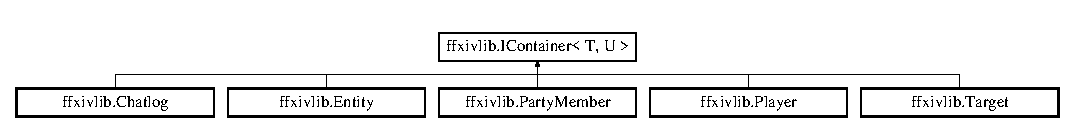
\includegraphics[height=1.341317cm]{classffxivlib_1_1_i_container_3_01_t_00_01_u_01_4}
\end{center}
\end{figure}
\subsection*{Public Member Functions}
\begin{DoxyCompactItemize}
\item 
void \hyperlink{classffxivlib_1_1_i_container_3_01_t_00_01_u_01_4_ae9081b3163d43d4d655dc72ea50b7a3d}{modify$<$ X $>$} (string field, X value)
\begin{DoxyCompactList}\small\item\em This function computes the address inside F\-F\-X\-I\-V process space to be modified for a given field and then modifies it. \end{DoxyCompactList}\item 
void \hyperlink{classffxivlib_1_1_i_container_3_01_t_00_01_u_01_4_adf190803540c072242e04f8380befc46}{refresh} ()
\begin{DoxyCompactList}\small\item\em This refreshes the instance It may have unexpected behavior if address changes. \end{DoxyCompactList}\end{DoxyCompactItemize}
\subsection*{Public Attributes}
\begin{DoxyCompactItemize}
\item 
\hypertarget{classffxivlib_1_1_i_container_3_01_t_00_01_u_01_4_a4c25b42d6bd8f3114947d137bea657c1}{Int\-Ptr {\bfseries address}}\label{classffxivlib_1_1_i_container_3_01_t_00_01_u_01_4_a4c25b42d6bd8f3114947d137bea657c1}

\item 
\hypertarget{classffxivlib_1_1_i_container_3_01_t_00_01_u_01_4_a4a077a13df5c84a292c1c03e05bc9ac7}{U {\bfseries structure}}\label{classffxivlib_1_1_i_container_3_01_t_00_01_u_01_4_a4a077a13df5c84a292c1c03e05bc9ac7}

\end{DoxyCompactItemize}


\subsection{Detailed Description}
Basic managed container for structures and other infos 


\begin{DoxyTemplParams}{Template Parameters}
{\em T} & Managed object type\\
\hline
{\em U} & Structure type\\
\hline
\end{DoxyTemplParams}


Name is misleading, this is not an Interface.

\subsection{Member Function Documentation}
\hypertarget{classffxivlib_1_1_i_container_3_01_t_00_01_u_01_4_ae9081b3163d43d4d655dc72ea50b7a3d}{\index{ffxivlib\-::\-I\-Container$<$ T, U $>$@{ffxivlib\-::\-I\-Container$<$ T, U $>$}!modify$<$ X $>$@{modify$<$ X $>$}}
\index{modify$<$ X $>$@{modify$<$ X $>$}!ffxivlib::IContainer< T, U >@{ffxivlib\-::\-I\-Container$<$ T, U $>$}}
\subsubsection[{modify$<$ X $>$}]{\setlength{\rightskip}{0pt plus 5cm}void ffxivlib.\-I\-Container$<$ T, U $>$.modify$<$ X $>$ (
\begin{DoxyParamCaption}
\item[{string}]{field, }
\item[{X}]{value}
\end{DoxyParamCaption}
)}}\label{classffxivlib_1_1_i_container_3_01_t_00_01_u_01_4_ae9081b3163d43d4d655dc72ea50b7a3d}


This function computes the address inside F\-F\-X\-I\-V process space to be modified for a given field and then modifies it. 


\begin{DoxyTemplParams}{Template Parameters}
{\em X} & Type of the value to modify, stick to base types\\
\hline
\end{DoxyTemplParams}

\begin{DoxyParams}{Parameters}
{\em field} & Name of the structure field to modify\\
\hline
{\em value} & Value to assign to field\\
\hline
\end{DoxyParams}
\hypertarget{classffxivlib_1_1_i_container_3_01_t_00_01_u_01_4_adf190803540c072242e04f8380befc46}{\index{ffxivlib\-::\-I\-Container$<$ T, U $>$@{ffxivlib\-::\-I\-Container$<$ T, U $>$}!refresh@{refresh}}
\index{refresh@{refresh}!ffxivlib::IContainer< T, U >@{ffxivlib\-::\-I\-Container$<$ T, U $>$}}
\subsubsection[{refresh}]{\setlength{\rightskip}{0pt plus 5cm}void ffxivlib.\-I\-Container$<$ T, U $>$.refresh (
\begin{DoxyParamCaption}
{}
\end{DoxyParamCaption}
)}}\label{classffxivlib_1_1_i_container_3_01_t_00_01_u_01_4_adf190803540c072242e04f8380befc46}


This refreshes the instance It may have unexpected behavior if address changes. 



The documentation for this class was generated from the following file\-:\begin{DoxyCompactItemize}
\item 
Interface.\-cs\end{DoxyCompactItemize}

\hypertarget{classffxivlib_1_1_party_member}{\section{ffxivlib.\-Party\-Member Class Reference}
\label{classffxivlib_1_1_party_member}\index{ffxivlib.\-Party\-Member@{ffxivlib.\-Party\-Member}}
}
Inheritance diagram for ffxivlib.\-Party\-Member\-:\begin{figure}[H]
\begin{center}
\leavevmode
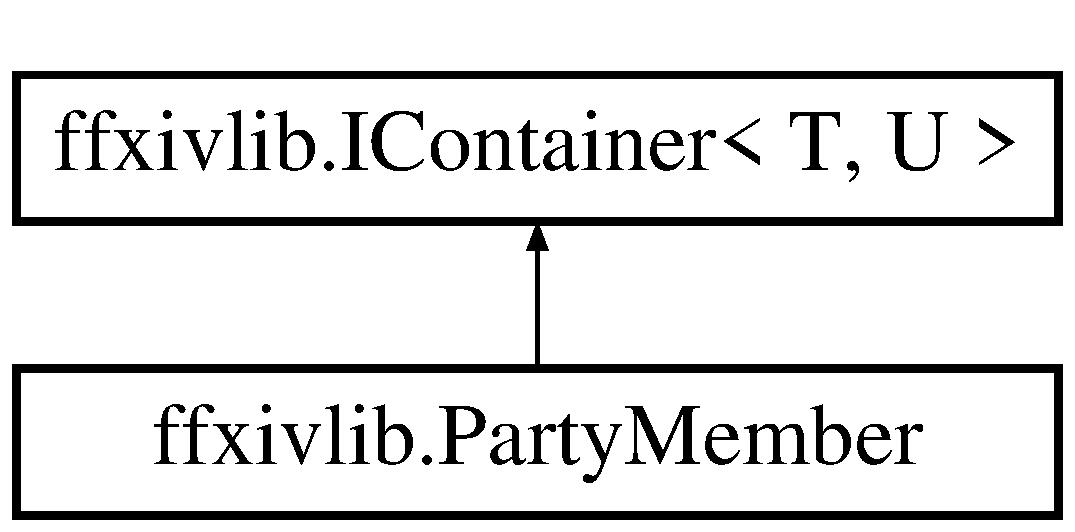
\includegraphics[height=2.000000cm]{classffxivlib_1_1_party_member}
\end{center}
\end{figure}
\subsection*{Classes}
\begin{DoxyCompactItemize}
\item 
struct \hyperlink{structffxivlib_1_1_party_member_1_1_p_a_r_t_y_m_e_m_b_e_r_i_n_f_o}{P\-A\-R\-T\-Y\-M\-E\-M\-B\-E\-R\-I\-N\-F\-O}
\end{DoxyCompactItemize}
\subsection*{Public Member Functions}
\begin{DoxyCompactItemize}
\item 
\hypertarget{classffxivlib_1_1_party_member_adc4a8b102bf341ca1dce3a2a7f92fa28}{{\bfseries Party\-Member} (\hyperlink{structffxivlib_1_1_party_member_1_1_p_a_r_t_y_m_e_m_b_e_r_i_n_f_o}{P\-A\-R\-T\-Y\-M\-E\-M\-B\-E\-R\-I\-N\-F\-O} \-\_\-structure, Int\-Ptr \-\_\-address)}\label{classffxivlib_1_1_party_member_adc4a8b102bf341ca1dce3a2a7f92fa28}

\end{DoxyCompactItemize}
\subsection*{Additional Inherited Members}


The documentation for this class was generated from the following file\-:\begin{DoxyCompactItemize}
\item 
Party\-Member.\-cs\end{DoxyCompactItemize}

\hypertarget{structffxivlib_1_1_party_member_1_1_p_a_r_t_y_m_e_m_b_e_r_i_n_f_o}{\section{ffxivlib.\-Party\-Member.\-P\-A\-R\-T\-Y\-M\-E\-M\-B\-E\-R\-I\-N\-F\-O Struct Reference}
\label{structffxivlib_1_1_party_member_1_1_p_a_r_t_y_m_e_m_b_e_r_i_n_f_o}\index{ffxivlib.\-Party\-Member.\-P\-A\-R\-T\-Y\-M\-E\-M\-B\-E\-R\-I\-N\-F\-O@{ffxivlib.\-Party\-Member.\-P\-A\-R\-T\-Y\-M\-E\-M\-B\-E\-R\-I\-N\-F\-O}}
}
\subsection*{Public Attributes}
\begin{DoxyCompactItemize}
\item 
\hypertarget{structffxivlib_1_1_party_member_1_1_p_a_r_t_y_m_e_m_b_e_r_i_n_f_o_a58cd6e399a19de16d25ddd42e8518144}{int {\bfseries Player\-I\-D}}\label{structffxivlib_1_1_party_member_1_1_p_a_r_t_y_m_e_m_b_e_r_i_n_f_o_a58cd6e399a19de16d25ddd42e8518144}

\item 
\hypertarget{structffxivlib_1_1_party_member_1_1_p_a_r_t_y_m_e_m_b_e_r_i_n_f_o_a4492548143962ad7df8b67a6002c6045}{string {\bfseries name}}\label{structffxivlib_1_1_party_member_1_1_p_a_r_t_y_m_e_m_b_e_r_i_n_f_o_a4492548143962ad7df8b67a6002c6045}

\item 
\hypertarget{structffxivlib_1_1_party_member_1_1_p_a_r_t_y_m_e_m_b_e_r_i_n_f_o_af10347eeb797e20f6de779bbbbadcff4}{J\-O\-B {\bfseries job}}\label{structffxivlib_1_1_party_member_1_1_p_a_r_t_y_m_e_m_b_e_r_i_n_f_o_af10347eeb797e20f6de779bbbbadcff4}

\item 
\hypertarget{structffxivlib_1_1_party_member_1_1_p_a_r_t_y_m_e_m_b_e_r_i_n_f_o_a89ee49f09068f4c061341b09a600f6fd}{byte {\bfseries level}}\label{structffxivlib_1_1_party_member_1_1_p_a_r_t_y_m_e_m_b_e_r_i_n_f_o_a89ee49f09068f4c061341b09a600f6fd}

\item 
\hypertarget{structffxivlib_1_1_party_member_1_1_p_a_r_t_y_m_e_m_b_e_r_i_n_f_o_aaf8131973fc3b9edb108d5b98e5edb78}{int {\bfseries c\-H\-P}}\label{structffxivlib_1_1_party_member_1_1_p_a_r_t_y_m_e_m_b_e_r_i_n_f_o_aaf8131973fc3b9edb108d5b98e5edb78}

\item 
\hypertarget{structffxivlib_1_1_party_member_1_1_p_a_r_t_y_m_e_m_b_e_r_i_n_f_o_abd323379e9c68fdac70c7ed6522eec5b}{int {\bfseries m\-H\-P}}\label{structffxivlib_1_1_party_member_1_1_p_a_r_t_y_m_e_m_b_e_r_i_n_f_o_abd323379e9c68fdac70c7ed6522eec5b}

\item 
\hypertarget{structffxivlib_1_1_party_member_1_1_p_a_r_t_y_m_e_m_b_e_r_i_n_f_o_a43d93e11b5dcabde1ebd4ec56c415f0e}{int {\bfseries c\-M\-P}}\label{structffxivlib_1_1_party_member_1_1_p_a_r_t_y_m_e_m_b_e_r_i_n_f_o_a43d93e11b5dcabde1ebd4ec56c415f0e}

\item 
\hypertarget{structffxivlib_1_1_party_member_1_1_p_a_r_t_y_m_e_m_b_e_r_i_n_f_o_ab45aa3bf2c4afd3991d11998154a3e11}{int {\bfseries m\-M\-P}}\label{structffxivlib_1_1_party_member_1_1_p_a_r_t_y_m_e_m_b_e_r_i_n_f_o_ab45aa3bf2c4afd3991d11998154a3e11}

\item 
\hypertarget{structffxivlib_1_1_party_member_1_1_p_a_r_t_y_m_e_m_b_e_r_i_n_f_o_a1c155a0c2169a8de7954c92dbf7ceb3c}{short {\bfseries c\-T\-P}}\label{structffxivlib_1_1_party_member_1_1_p_a_r_t_y_m_e_m_b_e_r_i_n_f_o_a1c155a0c2169a8de7954c92dbf7ceb3c}

\item 
\hypertarget{structffxivlib_1_1_party_member_1_1_p_a_r_t_y_m_e_m_b_e_r_i_n_f_o_adb063ab37768a38433ce89b80104e7b4}{short {\bfseries c\-G\-P}}\label{structffxivlib_1_1_party_member_1_1_p_a_r_t_y_m_e_m_b_e_r_i_n_f_o_adb063ab37768a38433ce89b80104e7b4}

\item 
\hypertarget{structffxivlib_1_1_party_member_1_1_p_a_r_t_y_m_e_m_b_e_r_i_n_f_o_a8bb33e0c66e5477b0dc1553c33da65c9}{short {\bfseries m\-G\-P}}\label{structffxivlib_1_1_party_member_1_1_p_a_r_t_y_m_e_m_b_e_r_i_n_f_o_a8bb33e0c66e5477b0dc1553c33da65c9}

\item 
\hypertarget{structffxivlib_1_1_party_member_1_1_p_a_r_t_y_m_e_m_b_e_r_i_n_f_o_a3fb2b0e1d689bff2f014f3a5c62c1b10}{float {\bfseries X}}\label{structffxivlib_1_1_party_member_1_1_p_a_r_t_y_m_e_m_b_e_r_i_n_f_o_a3fb2b0e1d689bff2f014f3a5c62c1b10}

\item 
\hypertarget{structffxivlib_1_1_party_member_1_1_p_a_r_t_y_m_e_m_b_e_r_i_n_f_o_a369a848b2aebd5fe73681193669aa2c5}{float {\bfseries Z}}\label{structffxivlib_1_1_party_member_1_1_p_a_r_t_y_m_e_m_b_e_r_i_n_f_o_a369a848b2aebd5fe73681193669aa2c5}

\item 
\hypertarget{structffxivlib_1_1_party_member_1_1_p_a_r_t_y_m_e_m_b_e_r_i_n_f_o_aa6de8771062f75d37ace78b480b2f981}{float {\bfseries Y}}\label{structffxivlib_1_1_party_member_1_1_p_a_r_t_y_m_e_m_b_e_r_i_n_f_o_aa6de8771062f75d37ace78b480b2f981}

\item 
\hypertarget{structffxivlib_1_1_party_member_1_1_p_a_r_t_y_m_e_m_b_e_r_i_n_f_o_a469840cdac04937ef2b9010b382d6f18}{int {\bfseries padding}}\label{structffxivlib_1_1_party_member_1_1_p_a_r_t_y_m_e_m_b_e_r_i_n_f_o_a469840cdac04937ef2b9010b382d6f18}

\end{DoxyCompactItemize}


The documentation for this struct was generated from the following file\-:\begin{DoxyCompactItemize}
\item 
Party\-Member.\-cs\end{DoxyCompactItemize}

\hypertarget{classffxivlib_1_1_player}{\section{ffxivlib.\-Player Class Reference}
\label{classffxivlib_1_1_player}\index{ffxivlib.\-Player@{ffxivlib.\-Player}}
}
Inheritance diagram for ffxivlib.\-Player\-:\begin{figure}[H]
\begin{center}
\leavevmode
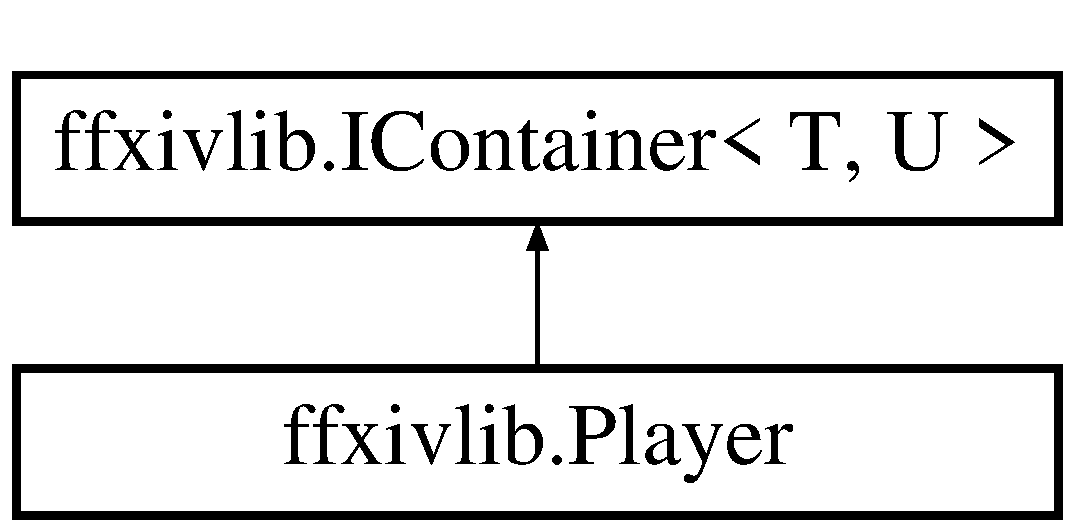
\includegraphics[height=2.000000cm]{classffxivlib_1_1_player}
\end{center}
\end{figure}
\subsection*{Classes}
\begin{DoxyCompactItemize}
\item 
struct \hyperlink{structffxivlib_1_1_player_1_1_p_l_a_y_e_r_i_n_f_o}{P\-L\-A\-Y\-E\-R\-I\-N\-F\-O}
\end{DoxyCompactItemize}
\subsection*{Public Member Functions}
\begin{DoxyCompactItemize}
\item 
\hypertarget{classffxivlib_1_1_player_a1ea21cf10a56fd9fef3bc4b0d54516bf}{{\bfseries Player} (\hyperlink{structffxivlib_1_1_player_1_1_p_l_a_y_e_r_i_n_f_o}{P\-L\-A\-Y\-E\-R\-I\-N\-F\-O} \-\_\-structure, Int\-Ptr \-\_\-address)}\label{classffxivlib_1_1_player_a1ea21cf10a56fd9fef3bc4b0d54516bf}

\end{DoxyCompactItemize}
\subsection*{Additional Inherited Members}


The documentation for this class was generated from the following file\-:\begin{DoxyCompactItemize}
\item 
Player.\-cs\end{DoxyCompactItemize}

\hypertarget{structffxivlib_1_1_player_1_1_p_l_a_y_e_r_i_n_f_o}{\section{ffxivlib.\-Player.\-P\-L\-A\-Y\-E\-R\-I\-N\-F\-O Struct Reference}
\label{structffxivlib_1_1_player_1_1_p_l_a_y_e_r_i_n_f_o}\index{ffxivlib.\-Player.\-P\-L\-A\-Y\-E\-R\-I\-N\-F\-O@{ffxivlib.\-Player.\-P\-L\-A\-Y\-E\-R\-I\-N\-F\-O}}
}
\subsection*{Public Attributes}
\begin{DoxyCompactItemize}
\item 
\hypertarget{structffxivlib_1_1_player_1_1_p_l_a_y_e_r_i_n_f_o_ac9fa36ba16ba6de0c095e719499e3161}{\hyperlink{namespaceffxivlib_a7273810711af045adb7151580e025a86}{J\-O\-B} {\bfseries Job}}\label{structffxivlib_1_1_player_1_1_p_l_a_y_e_r_i_n_f_o_ac9fa36ba16ba6de0c095e719499e3161}

\item 
\hypertarget{structffxivlib_1_1_player_1_1_p_l_a_y_e_r_i_n_f_o_a02da933d2d2a5fd52f48985c32766362}{byte {\bfseries P\-G\-L}}\label{structffxivlib_1_1_player_1_1_p_l_a_y_e_r_i_n_f_o_a02da933d2d2a5fd52f48985c32766362}

\item 
\hypertarget{structffxivlib_1_1_player_1_1_p_l_a_y_e_r_i_n_f_o_ae92ce14749b8bef22302c93f8b6fcc06}{byte {\bfseries G\-L\-D}}\label{structffxivlib_1_1_player_1_1_p_l_a_y_e_r_i_n_f_o_ae92ce14749b8bef22302c93f8b6fcc06}

\item 
\hypertarget{structffxivlib_1_1_player_1_1_p_l_a_y_e_r_i_n_f_o_a419071b0828fa14f989c7a658f77b581}{byte {\bfseries M\-R\-D}}\label{structffxivlib_1_1_player_1_1_p_l_a_y_e_r_i_n_f_o_a419071b0828fa14f989c7a658f77b581}

\item 
\hypertarget{structffxivlib_1_1_player_1_1_p_l_a_y_e_r_i_n_f_o_a8538e2e919f6735bd62c1e810148855f}{byte {\bfseries A\-R\-C}}\label{structffxivlib_1_1_player_1_1_p_l_a_y_e_r_i_n_f_o_a8538e2e919f6735bd62c1e810148855f}

\item 
\hypertarget{structffxivlib_1_1_player_1_1_p_l_a_y_e_r_i_n_f_o_a160d923c83dd5d1c3b94f0c402d92412}{byte {\bfseries L\-N\-C}}\label{structffxivlib_1_1_player_1_1_p_l_a_y_e_r_i_n_f_o_a160d923c83dd5d1c3b94f0c402d92412}

\item 
\hypertarget{structffxivlib_1_1_player_1_1_p_l_a_y_e_r_i_n_f_o_a19cfd8292fe579f506f0657f378af73c}{byte {\bfseries T\-H\-M}}\label{structffxivlib_1_1_player_1_1_p_l_a_y_e_r_i_n_f_o_a19cfd8292fe579f506f0657f378af73c}

\item 
\hypertarget{structffxivlib_1_1_player_1_1_p_l_a_y_e_r_i_n_f_o_a7068a8225f8b33d29ed30349c457267d}{byte {\bfseries C\-N\-J}}\label{structffxivlib_1_1_player_1_1_p_l_a_y_e_r_i_n_f_o_a7068a8225f8b33d29ed30349c457267d}

\item 
\hypertarget{structffxivlib_1_1_player_1_1_p_l_a_y_e_r_i_n_f_o_aca91a3431f24586c9d8411d1aec11255}{byte {\bfseries C\-P\-T}}\label{structffxivlib_1_1_player_1_1_p_l_a_y_e_r_i_n_f_o_aca91a3431f24586c9d8411d1aec11255}

\item 
\hypertarget{structffxivlib_1_1_player_1_1_p_l_a_y_e_r_i_n_f_o_abad29ae46b37fb8c038165b6b920eb83}{byte {\bfseries B\-S\-M}}\label{structffxivlib_1_1_player_1_1_p_l_a_y_e_r_i_n_f_o_abad29ae46b37fb8c038165b6b920eb83}

\item 
\hypertarget{structffxivlib_1_1_player_1_1_p_l_a_y_e_r_i_n_f_o_ab5374e952e3aa2bd71aa4de10cb21fe3}{byte {\bfseries A\-R\-M}}\label{structffxivlib_1_1_player_1_1_p_l_a_y_e_r_i_n_f_o_ab5374e952e3aa2bd71aa4de10cb21fe3}

\item 
\hypertarget{structffxivlib_1_1_player_1_1_p_l_a_y_e_r_i_n_f_o_a871754d40c5f17d780e85fa3e178c4e6}{byte {\bfseries G\-S\-M}}\label{structffxivlib_1_1_player_1_1_p_l_a_y_e_r_i_n_f_o_a871754d40c5f17d780e85fa3e178c4e6}

\item 
\hypertarget{structffxivlib_1_1_player_1_1_p_l_a_y_e_r_i_n_f_o_ab6d43c0c19945dd2352e76eaf8e98048}{byte {\bfseries L\-T\-W}}\label{structffxivlib_1_1_player_1_1_p_l_a_y_e_r_i_n_f_o_ab6d43c0c19945dd2352e76eaf8e98048}

\item 
\hypertarget{structffxivlib_1_1_player_1_1_p_l_a_y_e_r_i_n_f_o_a1376a72456ffac50ca345d53151aaf7e}{byte {\bfseries W\-V\-R}}\label{structffxivlib_1_1_player_1_1_p_l_a_y_e_r_i_n_f_o_a1376a72456ffac50ca345d53151aaf7e}

\item 
\hypertarget{structffxivlib_1_1_player_1_1_p_l_a_y_e_r_i_n_f_o_a4c61010475c50f40ef4ef9e3616e2e4c}{byte {\bfseries A\-L\-C}}\label{structffxivlib_1_1_player_1_1_p_l_a_y_e_r_i_n_f_o_a4c61010475c50f40ef4ef9e3616e2e4c}

\item 
\hypertarget{structffxivlib_1_1_player_1_1_p_l_a_y_e_r_i_n_f_o_af300af810373a6854c6057fdcb74a584}{byte {\bfseries C\-U\-L}}\label{structffxivlib_1_1_player_1_1_p_l_a_y_e_r_i_n_f_o_af300af810373a6854c6057fdcb74a584}

\item 
\hypertarget{structffxivlib_1_1_player_1_1_p_l_a_y_e_r_i_n_f_o_a3e21bdaa72143edbc1f2f7d27eca3cf0}{byte {\bfseries M\-I\-N}}\label{structffxivlib_1_1_player_1_1_p_l_a_y_e_r_i_n_f_o_a3e21bdaa72143edbc1f2f7d27eca3cf0}

\item 
\hypertarget{structffxivlib_1_1_player_1_1_p_l_a_y_e_r_i_n_f_o_a9fdb011f2e75c82891baf09c22b26c07}{byte {\bfseries B\-O\-T}}\label{structffxivlib_1_1_player_1_1_p_l_a_y_e_r_i_n_f_o_a9fdb011f2e75c82891baf09c22b26c07}

\item 
\hypertarget{structffxivlib_1_1_player_1_1_p_l_a_y_e_r_i_n_f_o_addc8a7d82af3f02b7d898bdb5b102cd5}{byte {\bfseries F\-S\-H}}\label{structffxivlib_1_1_player_1_1_p_l_a_y_e_r_i_n_f_o_addc8a7d82af3f02b7d898bdb5b102cd5}

\item 
\hypertarget{structffxivlib_1_1_player_1_1_p_l_a_y_e_r_i_n_f_o_a09c285b27f997415bbede248016cead7}{int {\bfseries P\-G\-L\-\_\-\-E\-I\-L}}\label{structffxivlib_1_1_player_1_1_p_l_a_y_e_r_i_n_f_o_a09c285b27f997415bbede248016cead7}

\item 
\hypertarget{structffxivlib_1_1_player_1_1_p_l_a_y_e_r_i_n_f_o_ac4e8c981f9b398ca7af3a6a51c764bfa}{int {\bfseries G\-L\-D\-\_\-\-E\-I\-L}}\label{structffxivlib_1_1_player_1_1_p_l_a_y_e_r_i_n_f_o_ac4e8c981f9b398ca7af3a6a51c764bfa}

\item 
\hypertarget{structffxivlib_1_1_player_1_1_p_l_a_y_e_r_i_n_f_o_ad67024737e35c0598cff9ee42022d697}{int {\bfseries M\-R\-D\-\_\-\-E\-I\-L}}\label{structffxivlib_1_1_player_1_1_p_l_a_y_e_r_i_n_f_o_ad67024737e35c0598cff9ee42022d697}

\item 
\hypertarget{structffxivlib_1_1_player_1_1_p_l_a_y_e_r_i_n_f_o_a44af95ee055a4d87d031be4865ba47f4}{int {\bfseries A\-R\-C\-\_\-\-E\-I\-L}}\label{structffxivlib_1_1_player_1_1_p_l_a_y_e_r_i_n_f_o_a44af95ee055a4d87d031be4865ba47f4}

\item 
\hypertarget{structffxivlib_1_1_player_1_1_p_l_a_y_e_r_i_n_f_o_a71a57bee66f5e505fcd48e46cc55160b}{int {\bfseries L\-N\-C\-\_\-\-E\-I\-L}}\label{structffxivlib_1_1_player_1_1_p_l_a_y_e_r_i_n_f_o_a71a57bee66f5e505fcd48e46cc55160b}

\item 
\hypertarget{structffxivlib_1_1_player_1_1_p_l_a_y_e_r_i_n_f_o_a6b3ee5daf97fbaf1d6629d512c5ee4c9}{int {\bfseries T\-H\-M\-\_\-\-E\-I\-L}}\label{structffxivlib_1_1_player_1_1_p_l_a_y_e_r_i_n_f_o_a6b3ee5daf97fbaf1d6629d512c5ee4c9}

\item 
\hypertarget{structffxivlib_1_1_player_1_1_p_l_a_y_e_r_i_n_f_o_a73e5646b9c4fc4cd732d36dd73054bb4}{int {\bfseries C\-N\-J\-\_\-\-E\-I\-L}}\label{structffxivlib_1_1_player_1_1_p_l_a_y_e_r_i_n_f_o_a73e5646b9c4fc4cd732d36dd73054bb4}

\item 
\hypertarget{structffxivlib_1_1_player_1_1_p_l_a_y_e_r_i_n_f_o_a18d03abb5c7cf635855bca2bb37129a3}{int {\bfseries A\-C\-N\-\_\-\-E\-I\-L}}\label{structffxivlib_1_1_player_1_1_p_l_a_y_e_r_i_n_f_o_a18d03abb5c7cf635855bca2bb37129a3}

\item 
\hypertarget{structffxivlib_1_1_player_1_1_p_l_a_y_e_r_i_n_f_o_ab8a1653ac3e6691193bccd813205ff70}{int {\bfseries B\-S\-M\-\_\-\-E\-I\-L}}\label{structffxivlib_1_1_player_1_1_p_l_a_y_e_r_i_n_f_o_ab8a1653ac3e6691193bccd813205ff70}

\item 
\hypertarget{structffxivlib_1_1_player_1_1_p_l_a_y_e_r_i_n_f_o_a2c5fa3956605e8ab10549174f6ec0b53}{int {\bfseries C\-P\-T\-\_\-\-E\-I\-L}}\label{structffxivlib_1_1_player_1_1_p_l_a_y_e_r_i_n_f_o_a2c5fa3956605e8ab10549174f6ec0b53}

\item 
\hypertarget{structffxivlib_1_1_player_1_1_p_l_a_y_e_r_i_n_f_o_adca9aa530e6c39a4bfa6ba5c55e81eee}{int {\bfseries G\-S\-M\-\_\-\-E\-I\-L}}\label{structffxivlib_1_1_player_1_1_p_l_a_y_e_r_i_n_f_o_adca9aa530e6c39a4bfa6ba5c55e81eee}

\item 
\hypertarget{structffxivlib_1_1_player_1_1_p_l_a_y_e_r_i_n_f_o_a1aed499022e07844d919ac221cd1a542}{int {\bfseries A\-R\-M\-\_\-\-E\-I\-L}}\label{structffxivlib_1_1_player_1_1_p_l_a_y_e_r_i_n_f_o_a1aed499022e07844d919ac221cd1a542}

\item 
\hypertarget{structffxivlib_1_1_player_1_1_p_l_a_y_e_r_i_n_f_o_ac99fd26cd862d2208f37918886d62b04}{int {\bfseries W\-V\-R\-\_\-\-E\-I\-L}}\label{structffxivlib_1_1_player_1_1_p_l_a_y_e_r_i_n_f_o_ac99fd26cd862d2208f37918886d62b04}

\item 
\hypertarget{structffxivlib_1_1_player_1_1_p_l_a_y_e_r_i_n_f_o_a5b5c5f9b4d0df8dfee036c7de6fb275f}{int {\bfseries L\-T\-W\-\_\-\-E\-I\-L}}\label{structffxivlib_1_1_player_1_1_p_l_a_y_e_r_i_n_f_o_a5b5c5f9b4d0df8dfee036c7de6fb275f}

\item 
\hypertarget{structffxivlib_1_1_player_1_1_p_l_a_y_e_r_i_n_f_o_a2af9cc134941566641728bbc3a9c0bd0}{int {\bfseries C\-U\-L\-\_\-\-E\-I\-L}}\label{structffxivlib_1_1_player_1_1_p_l_a_y_e_r_i_n_f_o_a2af9cc134941566641728bbc3a9c0bd0}

\item 
\hypertarget{structffxivlib_1_1_player_1_1_p_l_a_y_e_r_i_n_f_o_ac4c321134e1c976c624afa986349763f}{int {\bfseries M\-I\-N\-\_\-\-E\-I\-L}}\label{structffxivlib_1_1_player_1_1_p_l_a_y_e_r_i_n_f_o_ac4c321134e1c976c624afa986349763f}

\item 
\hypertarget{structffxivlib_1_1_player_1_1_p_l_a_y_e_r_i_n_f_o_a986af67bd72d62a2997d779cdac28f42}{int {\bfseries B\-O\-T\-\_\-\-E\-I\-L}}\label{structffxivlib_1_1_player_1_1_p_l_a_y_e_r_i_n_f_o_a986af67bd72d62a2997d779cdac28f42}

\item 
\hypertarget{structffxivlib_1_1_player_1_1_p_l_a_y_e_r_i_n_f_o_aa15b5819726cbb2a3b52fcdb536d959f}{int {\bfseries F\-S\-H\-\_\-\-E\-I\-L}}\label{structffxivlib_1_1_player_1_1_p_l_a_y_e_r_i_n_f_o_aa15b5819726cbb2a3b52fcdb536d959f}

\item 
\hypertarget{structffxivlib_1_1_player_1_1_p_l_a_y_e_r_i_n_f_o_a1ea1443ecebe63be94ccaabb22922293}{short {\bfseries Base\-S\-T\-R}}\label{structffxivlib_1_1_player_1_1_p_l_a_y_e_r_i_n_f_o_a1ea1443ecebe63be94ccaabb22922293}

\item 
\hypertarget{structffxivlib_1_1_player_1_1_p_l_a_y_e_r_i_n_f_o_a7c514757bd70d2b8b1e88e991e2e3041}{short {\bfseries Base\-D\-E\-X}}\label{structffxivlib_1_1_player_1_1_p_l_a_y_e_r_i_n_f_o_a7c514757bd70d2b8b1e88e991e2e3041}

\item 
\hypertarget{structffxivlib_1_1_player_1_1_p_l_a_y_e_r_i_n_f_o_a07de04293bb998c4aa804a70f9832e02}{short {\bfseries Base\-V\-I\-T}}\label{structffxivlib_1_1_player_1_1_p_l_a_y_e_r_i_n_f_o_a07de04293bb998c4aa804a70f9832e02}

\item 
\hypertarget{structffxivlib_1_1_player_1_1_p_l_a_y_e_r_i_n_f_o_a8f6b517d27385b927fee5d1d3b5ef9d2}{short {\bfseries Base\-I\-N\-T}}\label{structffxivlib_1_1_player_1_1_p_l_a_y_e_r_i_n_f_o_a8f6b517d27385b927fee5d1d3b5ef9d2}

\item 
\hypertarget{structffxivlib_1_1_player_1_1_p_l_a_y_e_r_i_n_f_o_a1b8922f0473320084043eba167130bbf}{short {\bfseries Base\-M\-N\-D}}\label{structffxivlib_1_1_player_1_1_p_l_a_y_e_r_i_n_f_o_a1b8922f0473320084043eba167130bbf}

\item 
\hypertarget{structffxivlib_1_1_player_1_1_p_l_a_y_e_r_i_n_f_o_aa729f65d1b57840aeaf8847690edb892}{short {\bfseries Base\-P\-I\-E}}\label{structffxivlib_1_1_player_1_1_p_l_a_y_e_r_i_n_f_o_aa729f65d1b57840aeaf8847690edb892}

\item 
\hypertarget{structffxivlib_1_1_player_1_1_p_l_a_y_e_r_i_n_f_o_ac75f17f8da60f245de7e857e9255f7e7}{short {\bfseries S\-T\-R}}\label{structffxivlib_1_1_player_1_1_p_l_a_y_e_r_i_n_f_o_ac75f17f8da60f245de7e857e9255f7e7}

\item 
\hypertarget{structffxivlib_1_1_player_1_1_p_l_a_y_e_r_i_n_f_o_ad1729b1ef3b9f9feb83a447783a5bc96}{short {\bfseries D\-E\-X}}\label{structffxivlib_1_1_player_1_1_p_l_a_y_e_r_i_n_f_o_ad1729b1ef3b9f9feb83a447783a5bc96}

\item 
\hypertarget{structffxivlib_1_1_player_1_1_p_l_a_y_e_r_i_n_f_o_a6246b16608d4f37003c51b0308ec6adb}{short {\bfseries V\-I\-T}}\label{structffxivlib_1_1_player_1_1_p_l_a_y_e_r_i_n_f_o_a6246b16608d4f37003c51b0308ec6adb}

\item 
\hypertarget{structffxivlib_1_1_player_1_1_p_l_a_y_e_r_i_n_f_o_af53def6a834b63cdeebaeff8237a5c9f}{short {\bfseries I\-N\-T}}\label{structffxivlib_1_1_player_1_1_p_l_a_y_e_r_i_n_f_o_af53def6a834b63cdeebaeff8237a5c9f}

\item 
\hypertarget{structffxivlib_1_1_player_1_1_p_l_a_y_e_r_i_n_f_o_ac9dfbeffa74bd0e144f6dde5a71b24b3}{short {\bfseries M\-N\-D}}\label{structffxivlib_1_1_player_1_1_p_l_a_y_e_r_i_n_f_o_ac9dfbeffa74bd0e144f6dde5a71b24b3}

\item 
\hypertarget{structffxivlib_1_1_player_1_1_p_l_a_y_e_r_i_n_f_o_a8bf094f4fab80e4c13d2c136da966f21}{short {\bfseries P\-I\-E}}\label{structffxivlib_1_1_player_1_1_p_l_a_y_e_r_i_n_f_o_a8bf094f4fab80e4c13d2c136da966f21}

\item 
\hypertarget{structffxivlib_1_1_player_1_1_p_l_a_y_e_r_i_n_f_o_a5e40804a2edd919abe8bb49d96a6ec51}{int {\bfseries Max\-H\-P}}\label{structffxivlib_1_1_player_1_1_p_l_a_y_e_r_i_n_f_o_a5e40804a2edd919abe8bb49d96a6ec51}

\item 
\hypertarget{structffxivlib_1_1_player_1_1_p_l_a_y_e_r_i_n_f_o_a364a83ce29cad0aa5747211d45efef96}{int {\bfseries Max\-M\-P}}\label{structffxivlib_1_1_player_1_1_p_l_a_y_e_r_i_n_f_o_a364a83ce29cad0aa5747211d45efef96}

\item 
\hypertarget{structffxivlib_1_1_player_1_1_p_l_a_y_e_r_i_n_f_o_ab08c439d6fa31a6fb2f528f25bcc4247}{int {\bfseries Max\-T\-P}}\label{structffxivlib_1_1_player_1_1_p_l_a_y_e_r_i_n_f_o_ab08c439d6fa31a6fb2f528f25bcc4247}

\item 
\hypertarget{structffxivlib_1_1_player_1_1_p_l_a_y_e_r_i_n_f_o_a1abe15e691ad65a1da162dcca73e29ff}{int {\bfseries Max\-G\-P}}\label{structffxivlib_1_1_player_1_1_p_l_a_y_e_r_i_n_f_o_a1abe15e691ad65a1da162dcca73e29ff}

\item 
\hypertarget{structffxivlib_1_1_player_1_1_p_l_a_y_e_r_i_n_f_o_a7c3dc6c5aec6f0f6f6147f042c991396}{int {\bfseries Max\-C\-P}}\label{structffxivlib_1_1_player_1_1_p_l_a_y_e_r_i_n_f_o_a7c3dc6c5aec6f0f6f6147f042c991396}

\item 
\hypertarget{structffxivlib_1_1_player_1_1_p_l_a_y_e_r_i_n_f_o_a40fe1afcbb58f2b9ab0e6a328d807a98}{short {\bfseries Parry}}\label{structffxivlib_1_1_player_1_1_p_l_a_y_e_r_i_n_f_o_a40fe1afcbb58f2b9ab0e6a328d807a98}

\item 
\hypertarget{structffxivlib_1_1_player_1_1_p_l_a_y_e_r_i_n_f_o_a28064adb3f1ff6e1803f744c6039df3c}{short {\bfseries Defense}}\label{structffxivlib_1_1_player_1_1_p_l_a_y_e_r_i_n_f_o_a28064adb3f1ff6e1803f744c6039df3c}

\item 
\hypertarget{structffxivlib_1_1_player_1_1_p_l_a_y_e_r_i_n_f_o_aa097eef225b35dd88452c6f893a5b327}{short {\bfseries Evasion}}\label{structffxivlib_1_1_player_1_1_p_l_a_y_e_r_i_n_f_o_aa097eef225b35dd88452c6f893a5b327}

\item 
\hypertarget{structffxivlib_1_1_player_1_1_p_l_a_y_e_r_i_n_f_o_aca8d6ee276da6dab7535dcdf26652053}{short {\bfseries Magic\-Defense}}\label{structffxivlib_1_1_player_1_1_p_l_a_y_e_r_i_n_f_o_aca8d6ee276da6dab7535dcdf26652053}

\item 
\hypertarget{structffxivlib_1_1_player_1_1_p_l_a_y_e_r_i_n_f_o_aa5f86c0049ea579da27d66cdd94fbb10}{short {\bfseries Slashing\-Res}}\label{structffxivlib_1_1_player_1_1_p_l_a_y_e_r_i_n_f_o_aa5f86c0049ea579da27d66cdd94fbb10}

\item 
\hypertarget{structffxivlib_1_1_player_1_1_p_l_a_y_e_r_i_n_f_o_a88401b4f067381001c94eb1e9437c05c}{short {\bfseries Piercing\-Res}}\label{structffxivlib_1_1_player_1_1_p_l_a_y_e_r_i_n_f_o_a88401b4f067381001c94eb1e9437c05c}

\item 
\hypertarget{structffxivlib_1_1_player_1_1_p_l_a_y_e_r_i_n_f_o_ae2dac563436cbd8c5e1b64f230d9a7e6}{short {\bfseries Blunt\-Res}}\label{structffxivlib_1_1_player_1_1_p_l_a_y_e_r_i_n_f_o_ae2dac563436cbd8c5e1b64f230d9a7e6}

\item 
\hypertarget{structffxivlib_1_1_player_1_1_p_l_a_y_e_r_i_n_f_o_a79877ac8a791aac8cc18e2a14bf64729}{short {\bfseries Fire\-Res}}\label{structffxivlib_1_1_player_1_1_p_l_a_y_e_r_i_n_f_o_a79877ac8a791aac8cc18e2a14bf64729}

\item 
\hypertarget{structffxivlib_1_1_player_1_1_p_l_a_y_e_r_i_n_f_o_a1056f3e044ca6455710d6233ae0abca5}{short {\bfseries Ice\-Res}}\label{structffxivlib_1_1_player_1_1_p_l_a_y_e_r_i_n_f_o_a1056f3e044ca6455710d6233ae0abca5}

\item 
\hypertarget{structffxivlib_1_1_player_1_1_p_l_a_y_e_r_i_n_f_o_a3c79a58ed35a09551a80199bb0c6e98b}{short {\bfseries Wind\-Res}}\label{structffxivlib_1_1_player_1_1_p_l_a_y_e_r_i_n_f_o_a3c79a58ed35a09551a80199bb0c6e98b}

\item 
\hypertarget{structffxivlib_1_1_player_1_1_p_l_a_y_e_r_i_n_f_o_afa5ca2d89e3c3ffc16ac03eaf302cbc7}{short {\bfseries Earth\-Res}}\label{structffxivlib_1_1_player_1_1_p_l_a_y_e_r_i_n_f_o_afa5ca2d89e3c3ffc16ac03eaf302cbc7}

\item 
\hypertarget{structffxivlib_1_1_player_1_1_p_l_a_y_e_r_i_n_f_o_a73deb027864acafcdb82bbb9d937e068}{short {\bfseries Lightning\-Res}}\label{structffxivlib_1_1_player_1_1_p_l_a_y_e_r_i_n_f_o_a73deb027864acafcdb82bbb9d937e068}

\item 
\hypertarget{structffxivlib_1_1_player_1_1_p_l_a_y_e_r_i_n_f_o_af9833ed275f9725436dace7f96ced3de}{short {\bfseries Water\-Res}}\label{structffxivlib_1_1_player_1_1_p_l_a_y_e_r_i_n_f_o_af9833ed275f9725436dace7f96ced3de}

\item 
\hypertarget{structffxivlib_1_1_player_1_1_p_l_a_y_e_r_i_n_f_o_afde1deb450feea6673850b787b0c1163}{short {\bfseries Attack\-Pow}}\label{structffxivlib_1_1_player_1_1_p_l_a_y_e_r_i_n_f_o_afde1deb450feea6673850b787b0c1163}

\item 
\hypertarget{structffxivlib_1_1_player_1_1_p_l_a_y_e_r_i_n_f_o_ab53527a666ee920f25350ff0e98f7265}{short {\bfseries Accuracy}}\label{structffxivlib_1_1_player_1_1_p_l_a_y_e_r_i_n_f_o_ab53527a666ee920f25350ff0e98f7265}

\item 
\hypertarget{structffxivlib_1_1_player_1_1_p_l_a_y_e_r_i_n_f_o_ab40c6badf25d237553667c6e8cd2204b}{short {\bfseries Crit\-Rate}}\label{structffxivlib_1_1_player_1_1_p_l_a_y_e_r_i_n_f_o_ab40c6badf25d237553667c6e8cd2204b}

\item 
\hypertarget{structffxivlib_1_1_player_1_1_p_l_a_y_e_r_i_n_f_o_a82a84c20248f3b4697cdc0efbe115aaf}{short {\bfseries Attack\-Mag\-Pot}}\label{structffxivlib_1_1_player_1_1_p_l_a_y_e_r_i_n_f_o_a82a84c20248f3b4697cdc0efbe115aaf}

\item 
\hypertarget{structffxivlib_1_1_player_1_1_p_l_a_y_e_r_i_n_f_o_aa3672b08ab0dcf943814b39adc3684de}{short {\bfseries Heal\-Mag\-Pot}}\label{structffxivlib_1_1_player_1_1_p_l_a_y_e_r_i_n_f_o_aa3672b08ab0dcf943814b39adc3684de}

\item 
\hypertarget{structffxivlib_1_1_player_1_1_p_l_a_y_e_r_i_n_f_o_a808248c6e0a41b393bdc2aae1874ea8e}{short {\bfseries Determination}}\label{structffxivlib_1_1_player_1_1_p_l_a_y_e_r_i_n_f_o_a808248c6e0a41b393bdc2aae1874ea8e}

\item 
\hypertarget{structffxivlib_1_1_player_1_1_p_l_a_y_e_r_i_n_f_o_ab311411afe59aa5562b5f122fe97ca78}{short {\bfseries Skill\-Speed}}\label{structffxivlib_1_1_player_1_1_p_l_a_y_e_r_i_n_f_o_ab311411afe59aa5562b5f122fe97ca78}

\item 
\hypertarget{structffxivlib_1_1_player_1_1_p_l_a_y_e_r_i_n_f_o_acfca12f84244ffa407a78af2914b63fc}{short {\bfseries Spell\-Speed}}\label{structffxivlib_1_1_player_1_1_p_l_a_y_e_r_i_n_f_o_acfca12f84244ffa407a78af2914b63fc}

\item 
\hypertarget{structffxivlib_1_1_player_1_1_p_l_a_y_e_r_i_n_f_o_a132cc5dcd38950cf69ba96092c9ff817}{short {\bfseries Craftmanship}}\label{structffxivlib_1_1_player_1_1_p_l_a_y_e_r_i_n_f_o_a132cc5dcd38950cf69ba96092c9ff817}

\item 
\hypertarget{structffxivlib_1_1_player_1_1_p_l_a_y_e_r_i_n_f_o_adda7db7f5b2a2b74875cb56243d16cf2}{short {\bfseries Control}}\label{structffxivlib_1_1_player_1_1_p_l_a_y_e_r_i_n_f_o_adda7db7f5b2a2b74875cb56243d16cf2}

\item 
\hypertarget{structffxivlib_1_1_player_1_1_p_l_a_y_e_r_i_n_f_o_a06313cc141a14de1f3bfc07470192a3a}{short {\bfseries Gathering}}\label{structffxivlib_1_1_player_1_1_p_l_a_y_e_r_i_n_f_o_a06313cc141a14de1f3bfc07470192a3a}

\item 
\hypertarget{structffxivlib_1_1_player_1_1_p_l_a_y_e_r_i_n_f_o_afaa389295165211145f21e766cf35ed7}{short {\bfseries Perception}}\label{structffxivlib_1_1_player_1_1_p_l_a_y_e_r_i_n_f_o_afaa389295165211145f21e766cf35ed7}

\item 
\hypertarget{structffxivlib_1_1_player_1_1_p_l_a_y_e_r_i_n_f_o_ac5b81a1932db348b0b8a8a4595b91302}{byte {\bfseries Padding}}\label{structffxivlib_1_1_player_1_1_p_l_a_y_e_r_i_n_f_o_ac5b81a1932db348b0b8a8a4595b91302}

\end{DoxyCompactItemize}


The documentation for this struct was generated from the following file\-:\begin{DoxyCompactItemize}
\item 
Player.\-cs\end{DoxyCompactItemize}

\hypertarget{class_current_target_1_1_program}{\section{Current\-Target.\-Program Class Reference}
\label{class_current_target_1_1_program}\index{Current\-Target.\-Program@{Current\-Target.\-Program}}
}


The documentation for this class was generated from the following file\-:\begin{DoxyCompactItemize}
\item 
test\-\_\-project/\-Test\-App/Program.\-cs\end{DoxyCompactItemize}

\hypertarget{class_modify_icon_1_1_program}{\section{Modify\-Icon.\-Program Class Reference}
\label{class_modify_icon_1_1_program}\index{Modify\-Icon.\-Program@{Modify\-Icon.\-Program}}
}


The documentation for this class was generated from the following file\-:\begin{DoxyCompactItemize}
\item 
Modify\-Icon/Program.\-cs\end{DoxyCompactItemize}

\hypertarget{structffxivlib_1_1_party_member_1_1_s_t_a_t_u_s_e_f_f_e_c_t}{\section{ffxivlib.\-Party\-Member.\-S\-T\-A\-T\-U\-S\-E\-F\-F\-E\-C\-T Struct Reference}
\label{structffxivlib_1_1_party_member_1_1_s_t_a_t_u_s_e_f_f_e_c_t}\index{ffxivlib.\-Party\-Member.\-S\-T\-A\-T\-U\-S\-E\-F\-F\-E\-C\-T@{ffxivlib.\-Party\-Member.\-S\-T\-A\-T\-U\-S\-E\-F\-F\-E\-C\-T}}
}
\subsection*{Public Attributes}
\begin{DoxyCompactItemize}
\item 
\hypertarget{structffxivlib_1_1_party_member_1_1_s_t_a_t_u_s_e_f_f_e_c_t_ac3eb20d02168470162192da9b6852159}{B\-U\-F\-F {\bfseries buff}}\label{structffxivlib_1_1_party_member_1_1_s_t_a_t_u_s_e_f_f_e_c_t_ac3eb20d02168470162192da9b6852159}

\item 
\hypertarget{structffxivlib_1_1_party_member_1_1_s_t_a_t_u_s_e_f_f_e_c_t_a123f3d9ee1d9db297df62737bdaf87c7}{int {\bfseries provider}}\label{structffxivlib_1_1_party_member_1_1_s_t_a_t_u_s_e_f_f_e_c_t_a123f3d9ee1d9db297df62737bdaf87c7}

\end{DoxyCompactItemize}


The documentation for this struct was generated from the following file\-:\begin{DoxyCompactItemize}
\item 
Party\-Member.\-cs\end{DoxyCompactItemize}

\hypertarget{classffxivlib_1_1_target}{\section{ffxivlib.\-Target Class Reference}
\label{classffxivlib_1_1_target}\index{ffxivlib.\-Target@{ffxivlib.\-Target}}
}
Inheritance diagram for ffxivlib.\-Target\-:\begin{figure}[H]
\begin{center}
\leavevmode
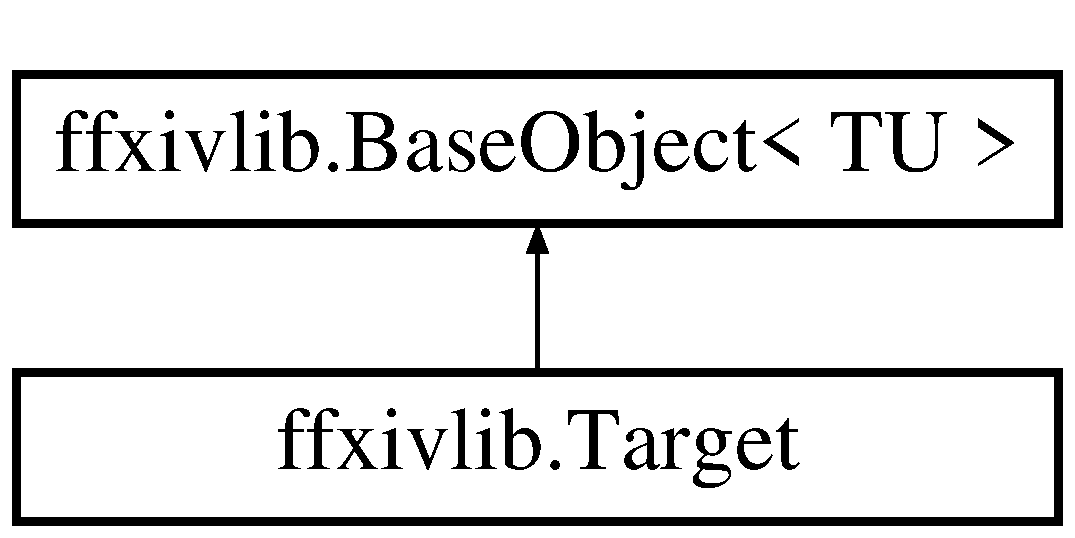
\includegraphics[height=2.000000cm]{classffxivlib_1_1_target}
\end{center}
\end{figure}
\subsection*{Classes}
\begin{DoxyCompactItemize}
\item 
struct \hyperlink{structffxivlib_1_1_target_1_1_t_a_r_g_e_t}{T\-A\-R\-G\-E\-T}
\end{DoxyCompactItemize}
\subsection*{Public Member Functions}
\begin{DoxyCompactItemize}
\item 
\hypertarget{classffxivlib_1_1_target_a5f88f56fa734de68261acd4b7ba1037b}{{\bfseries Target} (\hyperlink{structffxivlib_1_1_target_1_1_t_a_r_g_e_t}{T\-A\-R\-G\-E\-T} structure, Int\-Ptr address)}\label{classffxivlib_1_1_target_a5f88f56fa734de68261acd4b7ba1037b}

\end{DoxyCompactItemize}
\subsection*{Properties}
\begin{DoxyCompactItemize}
\item 
\hypertarget{classffxivlib_1_1_target_a7dc71e5dcda40dd3d2e1187c0322e832}{int {\bfseries Current\-Target}\hspace{0.3cm}{\ttfamily  \mbox{[}get, set\mbox{]}}}\label{classffxivlib_1_1_target_a7dc71e5dcda40dd3d2e1187c0322e832}

\item 
\hypertarget{classffxivlib_1_1_target_ab7ca016a549a6d2621010523ea2f4b9f}{int {\bfseries Mouseover\-Target}\hspace{0.3cm}{\ttfamily  \mbox{[}get, set\mbox{]}}}\label{classffxivlib_1_1_target_ab7ca016a549a6d2621010523ea2f4b9f}

\item 
\hypertarget{classffxivlib_1_1_target_af06247ed5e1779a1af050ad1ebdf0f9c}{int {\bfseries Focus\-Target}\hspace{0.3cm}{\ttfamily  \mbox{[}get, set\mbox{]}}}\label{classffxivlib_1_1_target_af06247ed5e1779a1af050ad1ebdf0f9c}

\item 
\hypertarget{classffxivlib_1_1_target_afec2ed018ca78d593b3c40b1bfd03c42}{int {\bfseries Previous\-Target}\hspace{0.3cm}{\ttfamily  \mbox{[}get, set\mbox{]}}}\label{classffxivlib_1_1_target_afec2ed018ca78d593b3c40b1bfd03c42}

\item 
\hypertarget{classffxivlib_1_1_target_a8af5ace3db90633c7961a381a24566cf}{int {\bfseries Current\-Target\-I\-D}\hspace{0.3cm}{\ttfamily  \mbox{[}get, set\mbox{]}}}\label{classffxivlib_1_1_target_a8af5ace3db90633c7961a381a24566cf}

\end{DoxyCompactItemize}


The documentation for this class was generated from the following file\-:\begin{DoxyCompactItemize}
\item 
Target.\-cs\end{DoxyCompactItemize}

\hypertarget{structffxivlib_1_1_target_1_1_t_a_r_g_e_t}{\section{ffxivlib.\-Target.\-T\-A\-R\-G\-E\-T Struct Reference}
\label{structffxivlib_1_1_target_1_1_t_a_r_g_e_t}\index{ffxivlib.\-Target.\-T\-A\-R\-G\-E\-T@{ffxivlib.\-Target.\-T\-A\-R\-G\-E\-T}}
}
\subsection*{Public Attributes}
\begin{DoxyCompactItemize}
\item 
\hypertarget{structffxivlib_1_1_target_1_1_t_a_r_g_e_t_a09363b015f76f3fe6835f2329afa340d}{int {\bfseries Current\-Target}}\label{structffxivlib_1_1_target_1_1_t_a_r_g_e_t_a09363b015f76f3fe6835f2329afa340d}

\item 
\hypertarget{structffxivlib_1_1_target_1_1_t_a_r_g_e_t_a9ae0253a6651d33195eb2705ed72dbe7}{int {\bfseries Mouseover\-Target}}\label{structffxivlib_1_1_target_1_1_t_a_r_g_e_t_a9ae0253a6651d33195eb2705ed72dbe7}

\item 
\hypertarget{structffxivlib_1_1_target_1_1_t_a_r_g_e_t_a41d18413ff458102ffa918feb5b52cbe}{int {\bfseries Focus\-Target}}\label{structffxivlib_1_1_target_1_1_t_a_r_g_e_t_a41d18413ff458102ffa918feb5b52cbe}

\item 
\hypertarget{structffxivlib_1_1_target_1_1_t_a_r_g_e_t_a7efad8c4a75fbd1089826763551b63be}{int {\bfseries Previous\-Target}}\label{structffxivlib_1_1_target_1_1_t_a_r_g_e_t_a7efad8c4a75fbd1089826763551b63be}

\item 
\hypertarget{structffxivlib_1_1_target_1_1_t_a_r_g_e_t_a5966d34fa56acb18f67d364d8fb5d9d2}{int {\bfseries Current\-Target\-I\-D}}\label{structffxivlib_1_1_target_1_1_t_a_r_g_e_t_a5966d34fa56acb18f67d364d8fb5d9d2}

\end{DoxyCompactItemize}


The documentation for this struct was generated from the following file\-:\begin{DoxyCompactItemize}
\item 
Target.\-cs\end{DoxyCompactItemize}

%--- End generated contents ---

% Index
\newpage
\phantomsection
\addcontentsline{toc}{part}{Index}
\printindex

\end{document}
